%%% TO DO  as of 12/29/11

 %%% Spell check document
 %%% ?all-zero? should be all-zero and not all zero ?all zero? ?all 0? etc..
 %%% Fix up R scripts and consolidate for R package
 %%% R commands to process wolverine data need included in that section

 %%% Run Wolverine 2k 4k and 8k grids in JAGS compare to WinBUGS
 %%%     insert those results in text

 %%%  For discrete state-space stuff, convert BUGS output to JAGS and
 %%%  figure out MC errors
 %%% Finish Table that has those results in it



\chapter{Fully Spatial Capture-Recapture Models}
\markboth{Basic SCR Model}{}
\label{chapt.scr0}

\vspace{.3in}

In the previous chapter, we discussed models that could be
viewed as primitive spatial capture-recapture models. We looked at a
basic distance sampling model and we also considered a classical
individual covariate modeling approach in which we defined a covariate
to be the distance from the (estimated) home range center to the center of
the trap array. These were spatial in the sense that they included
some characterization of where individuals live but, on the other
hand, only a primitive or no characterization of trap location.  That
said, there is only a small step from these two models to spatial
capture-recapture models that we consider in this chapter, which fully
recognize the spatial attribution of both individual animals {\it and}
the locations of encounter devices.

Fully spatial capture-recapture models must accommodate the spatial
organization of individuals and the encounter devices because the
encounter process occurs at the level of individual traps.  Failure to
consider the trap-specific data is the key deficiency
with classical ad-hoc approaches which aggregate encounter information
to the resolution of the entire trap array. We have  previously
addressed some problems that this induces including induced
heterogeneity in encounter probability, imprecise notation of ``sample
area'' and not being able to accommodate trap-specific
effects or trap-specific missing values.
In this chapter we resolve these issues by developing 
our first fully spatial capture-recapture
model. This model is not too different from
that considered in sec. \ref{closed.sec.indcov} but, 
instead of defining the individual covariate to be distance
to the centroid of the array we define $J$ individual covariates - the
distance to {\it each} trap. And, instead of using estimates of
individual locations ${\bf s}$, we consider a fully hierarchical model in
which we regard ${\bf s}$ as a latent variable and impose a prior
distribution on it.  

In the following sections of this chapter we investigate the basic
spatial capture-recapture model, which we refer to as ``model SCR0'',  and address some important
considerations related to its analysis in {\bf BUGS}. 
We demonstrate
how to summarize posterior output for the purposes of producing
density maps or spatial predictions of density.
The key aspect of the SCR models considered in this chapter is the
formulation of a model for encounter probability that is a function of
distance between individual home range center and trap locations. 
We also discuss how encounter probability models are related to
explicit models of space usage or ``home range area.'' Understanding
this allows us to compute, for example, the area used by an individual
some prescribed percent of the time.  While it is intuitive that SCR
models should be related to a basic model of space usage, this
has not been discussed explicitly in the literature in any substantial
except by \citep{royle_chandler:2012} which we address further in
Chapt. \ref{chapt.rsf}. 




\section{Sampling Design and Data Structure}

In our development here, we will assume a standard sampling design in
which an array of $J$ traps is operated for $K$ time periods (say,
nights) producing encounters of $n$ individuals.  
Because sampling
occurs by traps and also over time, the most general data structure
yields encounter histories for {\it each individual} that are
temporally {\it and} spatially indexed. Thus a typical data set will
include an encounter history {\it matrix} for each individual
indicating which trap the individual was captured, during each sample occasion.  
For example, suppose we observe 6
individuals in sampling at 4 traps over 3 nights of sampling then a
plausible data set for a single individual captured one time in trap 1
on the first night and one time in trap 3 on the 3rd night is:
\begin{verbatim}
       night1 night2 night3
 trap1    1     0     0    
 trap2    0     0     0    
 trap3    0     0     1    
 trap4    0     0     0    
\end{verbatim}
This data structure would be obtained for {\it each} of the
$i=1,2,\ldots,n$ captured individuals. 

We develop models in this chapter for passive detection 
devices such as ``hair snares''
or other DNA sampling methods \citep{kery_etal:2010,
  gardner_etal:2010jwm} and related types of sampling devices in which
(i) devices (effective ``traps'') may capture any number of individuals (i.e.,
they don't fill up; \begin{comment}
This is referred to as a ``multi-catch'' type of
sampling \citep{efford_etal:2009ecol})\end{comment}; (ii) an individual may be
captured in more than one trap during each occasion but (iii) 
individuals can be encountered at most 1 time by each trap during any
occasion.  Hair snares for sampling DNA from bears and other species
function according to these rules. An individual bear wandering about
its territory might come into contact with  $>1$ devices; A device may
encounter multiple bears; However, in practice, it will often not be 
possible to attribute multiple visits of the same individual to
distinct encounter events.
While the model is most directly relevant
to hair snares and other DNA sampling methods for which multiple
detections of an individual are not distinguishable,
we will also make use of the model for data that arise from
camera-trapping studies. In practice, with camera trapping,
individuals might be photographed several times in a night but it is
common to 
 distill such data into a single binary encounter event for
reasons discussed later in Chapt. \ref{chapt.poisson-mn}.

%We will see shortly that the statistical model for these data is a
%binomial model with sample size $K=3$ and ``success probability'' $p$
%which depends on individual and trap. 
The statistical assumptions we make to build a model for these data 
are that individual encounters
within and among traps are independent, and this allows us to regard
individual- and trap-specific encounters as {\it independent} Bernoulli trials
(see next section).  These basic (but admittedly at this point
somewhat imprecise) assumptions define the basic spatial
capture-recapture model, which we will refer to as ``SCR0'' 
so that we may use that model as a point of reference without having
to provide a long-winded enumeration of assumptions and sampling
design each time we do. We will make things more precise as we develop
a formal statistical definition of the model shortly.


\section{The binomial encounter model}

We begin by considering the simplest possible model in which 
there are no time-varying covariates that
influence encounter, there are no explicit individual-specific
covariates, and there are no covariates that influence density. In
this case, we can aggregate the binary encounters over
the $K$ sample occasions and record the total number of encounters out
of $K$. We will denote these individual- and trap-specific encounter
frequencies by $y_{ij}$ for $i=1,2,\ldots,n$ captured
individuals and $j=1,2,\ldots,J$ traps.
For example, suppose we observe 6
individuals in sampling at 4 traps over 3 nights of sampling then a
plausible data set is the $6 \times 4$ matrix of encounters, out of 3,
of the form:
\begin{verbatim}
      trap1 trap2 trap3 trap4
 [1,]     1     0     0     0
 [2,]     0     2     0     0
 [3,]     0     0     0     1
 [4,]     0     1     0     0
 [5,]     0     0     1     1
 [6,]     1     0     1     0
\end{verbatim}
%If sampling devices are operated over $K$ time periods or sampling
%occasions (e.g., in practice,
%nights), and we assume that individual encounters are independent
%across the $K$ sampling occasions, so that   
% individual and trap-specific encounters, $y_{ij}$,
We assume that $y_{ij}$ are 
 mutually independent outcomes of a binomial random variable:
\begin{equation}
	y_{ij} \sim \mbox{Bin}(K, p_{ij})
\label{scr0.eq.bin}
\end{equation}
This is the basic model underlying
 standard closed population models
(Chapt. \ref{chapt.closed}) except that, in the present case, the
encounter probability $p_{ij}$ depends on both individual {\it and}
trap. 
%In a sense, then, we can think of each {\it trap} as producing individual
%level encounter history data of the classical variety - an $\mbox{\tt
%  nind} \times \mbox{\tt nreps}$ matrix of 0's and 1's (this is the
%``encountered at most 1 time'' assumption).


As we did in sec. \ref{closed.sec.indcov}, we will make explicit the
notion that $p_{ij}$ is defined conditional on {\it where} individual
$i$ lives. Naturally, we think about defining an individual home range
and then relating $p_{ij}$ explicitly to the centroid of the
individuals home range, or its center of activity \citep{efford:2004,
  borchers_efford:2008, royle_young:2008}.  Therefore, define ${\bf
  s}_{i}$, a two-dimensional spatial coordinate, to be the home range
or activity
center of individual $i$. Then, the SCR model postulates that
encounter probability, $p_{ij}$, is a decreasing function of distance
between ${\bf s}_{i}$ and the location of trap $j$, ${\bf x}_{j}$.
Naturally, if we think of modeling binomial counts using logistic
regression, with a model for $p_{ij}$ such as:
\begin{equation}
	\mbox{logit}(p_{ij}) = \alpha_{0} + \alpha_1 ||{\bf s}_{i}-{\bf x}_{j} ||
\label{scr0.eq.logit}
\end{equation}
where, here, $||{\bf s}_{i}-{\bf x}_{j}||$ is the distance between
${\bf s}_{i}$ and ${\bf x}_{j}$. We sometimes write $||{\bf
  s}_{i}-{\bf x}_{j}|| = dist({\bf s}_{i},{\bf x}_{j}) =
d_{ij}$.
We probably expect that the parameter $\alpha_{1}$ in
Eq. \ref{scr0.eq.logit} or \ref{scr0.eq.norm} should be negative, so
that the probability of encounter decreases with distance between the
trap and individual home range center.  

Alternatively, a popular model in distance sampling is:
\begin{equation}
p_{ij} = p_{0}*\exp(-\alpha_{1} *||{\bf s}_{i}-{\bf x}_{j}||^2)
\label{scr0.eq.norm}
\end{equation}
which is usually referred to as the ``half-normal'' model,
with $\alpha_{1} = 1/(2\sigma^{2})$.  Because it
is the kernel of a bivariate normal or Gaussian probability density
function we will refer to it as the ``(bivariate) normal'' or
``Gaussian'' model.  There are a large number of standard detection
models commonly used, and we consider these in
Chapt. \ref{chapt.covariates}. 
% Note that the bivariate normal model
%is equivalently represented as
%\begin{equation}
%\log(p_{ij})  = \log(p_{0}) - \alpha_{1} *||{\bf s}_{i}-{\bf x}_{j}||^2
%\label{scr0.eq.norm}
%\end{equation}
%which we make use of sometimes in specifying the model in the \bugs language. 
%We would always like to be clear that encounter probability depends on individual activity
%centers {\it and} trap locations {\it and} parameter(s) $\theta$, and
%so it would be ideal to write $p({\bf s}_{i},{\bf x}_{j}; \theta)$ or
%something similar. However, this can be extremely unwieldy and
%clutter up what are otherwise extremely simple mathematical
%expressions and formulae. As such, we will usually abbreviate these
%various dependencies by writing $p_{ij}$ or sometimes $p_{\theta,ij}$,
%understanding that $p_{ij}$ is actually a function of the various important
%quantities.

Whatever model we choose for encounter probability, we should always keep
in mind that the model is described conditional on ${\bf s}_{i}$,
which is an unobserved random variable.  Thus, to be precise about
this, we should write the observation model as
\[
y_{ij}|{\bf s}_{i} \sim \mbox{Bin}(K, p({\bf s}_{i};\alpha_{1}))
\]
but sometimes for notational simplicity we omit the latent variables
${\bf s}_{i}$.

\begin{comment}
The joint likelihood for the
data, conditional on the collection of individual activity centers,
can be expressed as
\[
{\cal L}(\alpha_{1} | \{ {\bf y}_{i},{\bf s}_{i} \}_{i=1}^{N})
 =  \prod_{i} \prod_{j} \mbox{Bin}(y_{ij}|p_{ij}(\alpha_{1}))
\]
If we switch the indices on the product operators, we recognize that SCR likelihood (conditional on ${\bf s}$) is the product of $J$
{\it independent} capture-recapture likelihoods - one for each trap.
However, the data have a distinct ``repeated measures'' type of structure, with
each of the $j$ likelihood contributions for each individual being
grouped by individual. Thus, we cannot analyze the model
meaningfully by $J$ trap-specific models. In classical repeated measures
types of models, we accommodate the group structure of the data using
random effects (random individual or group level variables). For SCR
models we take the same basic approach, which we develop subsequently.
\end{comment}



\subsection{Definition of home range center}

Some will be offended by our use of the concept of ``home range
center'' and question whether such notions as home ranges are useful
for some (or perhaps {\it any}) particular species.  Indeed, the idea
of a home range is a vague and purely phenomenological construct
anyway.  Despite this, it doesn't really matter whether or not a home
range makes sense for a particular species - individuals of any
species inhabit {\it some} region of space and we can define the
home range center to be the center of the space that individual
was occupying (or using) during the period in which traps were
active. Thinking about it in that way, it could even be observable
(almost) as the centroid of a very large number of radio fixes over
the course of a survey period or a season.  Thus, this practical
version of a home range center in terms of space usage is a
well-defined construct regardless of whether one thinks the home range
itself is a meaningful concept, even if individuals are not
particularly territorial.  This is why we usually use the term
``activity center'' and we recognize that this is a transient thing
which applies only to a well-defined period of study.
%See sec. \ref{sec.scr0.implied} for more discussion of how to 
%interpret ${\bf s}$ in the context of the detection probability
%model. 


\subsection{Distance as a latent variable}

If we knew precisely every ${\bf s}_{i}$ in the population (and
population size $N$), then the model specified by
eqs. \ref{scr0.eq.bin} and \ref{scr0.eq.logit} would be just an
ordinary logistic regression-type of a model which we learned how to
fit using {\bf WinBUGS} previously (Chapt. \ref{chapt.glms}), with a
covariate $d_{ij}$. However, the activity centers are unobservable
even in the best possible circumstances. In that case, $d_{ij}$ is an
unobserved variable, as in classical random effects models. We need to
therefore extend the model to accommodate these random variables with
an additional model component. A standard, and perhaps not
unreasonable, assumption is the so-called ``uniformity assumption''
which is to say that the ${\bf s}_{i}$ are uniformly distributed over
space (the obvious next question ``which space?'' is addressed below).
This uniformity assumption amounts to a uniform prior distribution on
${\bf s}_{i}$, i.e., the pdf of ${\bf s}_{i}$ is constant, which we
may express
\begin{equation}
	\Pr({\bf s}_{i}) \propto \mbox{\tt const}
\label{scr0.eq.sprior}
\end{equation}
 As it turns out, this assumption is usually not precise
enough to fit SCR models in practice for reasons we discuss in the
following section.  We will give another way to represent this prior
distribution that is more concrete, but depends on specifying the
``state-space'' of the random variable ${\bf s}_{i}$. The term
state-space is a technical way of saying ``the space of all possible
outcomes'' of the random variable.

To summarize the preceeding model developing, a basic SCR model is
defined by 3 essential components:
\begin{itemize}
\item[(1)] Observation model: $y_{ij}|{\bf s}_{i} \sim \mbox{Bin}(K, p_{ij})$
\item[(2)] Encounter probability model, such as: 
$p_{ij} = p_{0}*\exp(-\alpha_{1} *||{\bf s}_{i}-{\bf x}_{j}||^2)$
\item[(3)] Point process model: $\Pr({\bf s}_{i} ) \propto \mbox{\tt const}$
\end{itemize}
Therefore, the SCR model is little more than an ordinary
capture-recapture model for closed populations. It is such a model,
but augmented with a set of ``individual effects'', ${\bf s}_{i}$,
which relate some sense of individual location to encounter
probability. 

\subsection{The Core SCR Assumptions}

Its always a good idea to sit down and reflect on the meaning of any
particular model, its various assumptions, and what they mean in a
specific context.  From the statisticians point of view, the basic
assumption, the omnibus assumption, as in all of statistics, and for
every statistical model, is that ``the model is correctly
specified''. So, naturally, that precludes everything that isn't
explicitly addressed by the model.
 To point this out to someone seems to cause a lot of
anxiety, so we enumerate here what we think are the most important things
not accounted for by the model:

\begin{itemize} 
\item[$\bullet$] {\bf Demographic closure}. The model does not allow for demographic processes.
There is no recruitment or entry into the sampled population. There is 
no mortality or exit from the sampled population.
\item[$\bullet$] {\bf Geographic closure}?
 Strictly speaking this is not assumed -- animals may move around in
 space and sometimes be exposed to trapping and sometimes not. The
 whole point of SCR models is to accommodate this dynamic. In ordinary
 capture-recapture models we have to assume geographic closure to interpret $N$ in a
 meaningful way. Even with SCR models we can't simply assert that a
 lack of geographic closure is ok, because the model only accommodates
 a certain type of movement -- that of a central place forager.
\item[$\bullet$] {\bf Activity centers are randomly distributed}. That
  is, uniformity and independence of the underlying point
  process ${\bf s}_{1},\ldots, {\bf s}_{N}$.
\item[$\bullet$] {\bf Detection is a function of distance}. 
A detection model that provides a phenomonological
  description of how encounter probability varies as a function of distance.
 We are not making an explicit assumption about home range geometry or
 size, although a certain view leads naturally to such an
 interpretation. See the next section. 
\item[$\bullet$] {\bf Independence of encounters} among individuals.
\item[$\bullet$] {\bf Independence of encounters} of the same individual.
\end{itemize}
Its easy to get worried and question some of these assumptions just on
the grounds that they're so outrageously simple. But its worth
emphasizing here that you don't have inherently fewer assumptions by
using an ordinary capture-recapture problem but, rather, you have to
make more extravagent claims about what your data represent to
discregard certain aspects of the problem.  For one, we're not
assuming that $p$ is constant for all individuals but rather that $p$
varies substantially as a matter of spatial juxtaposition of
individuals with traps. So maybe the manner in which $p$ varies isn't
quite right, but whether or not we have that right, that is not an
argument for assuming $p$ to be constant or that, instead, it must
vary according to a 2-point finite mixture.  Fundamentally a
distance-based model for $p$ has some basic biological justification
for virtually all species that we study.

For some of these core assumptions, uniformity, isotropic/stationary
space usage, independence of individuals and of encounters, we expect
a fair amount of robustness to departures, for good reasons but,
importantly, we can extend these assumptions in many different ways
and we do that to varying extents in this book and more work remains 
to be done in this regard. We can also evaluate the reasonableness of the assumptions
formally in some cases using standard methods of assessing model fit
(Chapt. \ref{chapt.gof}).



\begin{comment}
We also note that having made these assumptions we shouldn't regard
them as completely definitive and necessary. For example, {\it your} inability to relax these
assumptions by generalizing the model should not be interpreted as
an an inability that applies to {\it everyone}. 

Finally, we return back to our sentiment about the omnibus assumptions
which is that the model is properly specified. This precludes
everything that isn't in the model. As a result of this, you sometimes
see in historical capture-recapture literature things like we assume
``no marks are lost'', we assume that ``marks are correctly
identified'' and so forth. We might as well also assume that, a
shopping mall is not built in our study area, a meteor does not crash
down into our study area, the sun does not go super-nova, and things
like that. Our point is that we should seperate statistical
assumptions about model parameters from what are essentially
logistical or operational assumptions about how we interpret our data
based on our ability to collect data. It is pointless to enumerate all
of the possible explanations for apparent {\it departures}, because
there are an infinity of such cases.
\end{comment}


\section{The Implied Model of Space Usage}
\label{sec.scr0.implied}


% bivariate normal a null model for "central place forager" but even
% for a non-central place foragter, the activity center is a transient
% thing so it produces an approximation over a short period.
% whilt it is a simple model we only have sparse movement observations
% in virtually all practical c-r situations
We developed the basic SCR model in terms of a latent variable, ${\bf
  s}$, the home range center or activity center.  Surely then, the
encounter probability model which relates encounter of individuals in
specific traps to ${\bf s}$ must somehow imply a certain model for
home range geometry and size -- ``space usage''.  Here we explore the
nature of that relationship and we argue that any given detection
model implies a model of space usage -- i.e., the amount and extent of
area used some prescribed percentage of the time. So we might say,
for example, 95\% of animal movements are within some distance from an
individual's activity center.  While we have used the term ``home
range'' or similar, what we really mean to imply is something that
would be more more clearly identified as space usage or
 resource selection. If the resource is only
homogeneous space, then space usage is a more descriptive term but,
otherwise (Chapt. \ref{chapt.rsf}) we take on the more genereal
problem of modeling resource selection.


Intuitively, the detection function of SCR models is related to home
range area or space usage of individuals.  Indeed, it is natural
to interpret the detection model as the composite of two processes:
movement of an individual about its home range i.e., how it uses space
within its home range (``space usage''), and detection {\it
  conditional on use} in the vicinity of a trapping device.
Formally we decompose encounter probability according to:
\[
 \Pr(\mbox{encounter at } {\bf x}|{\bf s})
 = \Pr(\mbox{encounter } | \mbox{usage of } {\bf x}, {\bf s}) 
\Pr(\mbox{usage of } {\bf x}|{\bf s}).
\]
In practice it might make sense to think about the first component,
i.e., $\Pr(\mbox{encounter} | \mbox{usage of} {\bf x}, {\bf s})$ as
being a constant (e.g., if traps are located within arbitrarily small
grid cells) and then, in that case, the encounter probability model is
directly proportional to this model for individual movements about
their home range center determining the use frequency of each ${\bf x}$.
This is a sensible heuristical model for what ecologists would call a
central place forager although we have stated previously that it may
be meaningful as a description of transient space usage as well. 

To motivate a specific model for space usage, imagine some kind of
perfect observation device (e.g., continuous telemetry) so that we
observe every time an individual moves into a pixel. After a long
period of time we observe an enormous sample size of ${\bf x}$
values. We tally those up into each pixel, producing the frequency
$m({\bf x},{\bf s})$, so then the usage model should be regarded as a probability
mass function for these counts. Naturally, we regard the counts
$m({\bf x},{\bf s})$
as a multinomial observation with probabilities $\pi({\bf x}|{\bf s})$ and
prescribe a suitable model for $\pi({\bf x}|{\bf s})$ that describes how use
events should accumulate over time. A natural null model for
$\pi({\bf x}|{\bf s})$ has a decreasing probability of use as ${\bf x}$ gets far away
from ${\bf s}$.  We could say that the points used by the individual
with activity center ${\bf s}$ represent a point process with 
conditional intensity:
\[
\pi({\bf x}|{\bf s}) =  \frac{ k({\bf x},{\bf s}) }{ \int k({\bf
    x},{\bf s}) dx }
\]
or, if we represent our landscape by discrete pixels, 
\begin{equation}
\pi({\bf x}|{\bf s}) =  \frac{ k({\bf x},{\bf s}) }{ \sum_{x} k({\bf
    x},{\bf s}) }
\label{scr0.eq.ud}
\end{equation}
where $k({\bf x},{\bf s})$ is any positive function. In continuous
space, we would just replace the denominator with an integral, but the
discrete space formulation of this is relevant to most practical
problems.
%This is the
%conditional intensity function of a point processes 
% looks like a
% type of resource selection function (RSF) 
%\citep[e.g.,][Ch. 8]{manly_etal:2001}.
Clearlythe space used by an individual will be proportional
to whatever kernel we stick in for the numerator. 
In the 
resource selection function (RSF) literature, a certain type of RSF
arises if we use 
a  negative exponential function \citep[e.g.,][Ch. 8]{manly_etal:2001}.
But, here we use a Gaussian kernel, i.e., 
\[
 k({\bf x},{\bf s})= \exp(  -d({\bf x},{\bf s})^{2}/(2\sigma^{2})) 
\]
so that space usage occurs according to a a bivariate normal model.

To apply
this model of space-usage to SCR problems we just allow for imperfect
detection by introducing a constant encounter rate $<1$, then this
yields, precisely, our bivariate normal encounter probability model.
The main take-away point here is that underlying every SCR model is
some kind of model of space-usage Eq. (\ref{scr0.eq.ud}) based on the
specific choice of $k({\bf x},{\bf s})$.  
Whether or not we have perfect sampling devices, the function we use
in the encounter probability model equates to some conditional
distribution of points, or utilization distribution, as in
Eq. \ref{scr0.eq.ud}, from which we can compute effective home range
area, i.e., the area that contains 95\% of the mass of $k({\bf x},{\bf
  s})$, or 95\% of all space used.


\begin{comment}
Whether or not a 
point $x$ is {\it used} (at all) depends on some unknown rate of use
by the individual over whatever period of time the devices are
active. This is something we can't hope to estimate or model in most
cases but we imagine that over a period of time usage is characterized
by a rate of usage $\lambda_{0}$ so that amount of usage -- the number
of times individual $s$ enters $x$, is:
\[
m({\bf x},{\bf s}) = Poisson(\lambda_{0} \pi(x|s) ) 
\]
which isn't really an important assumption because note that by
conditioning on the total again it retains the (natural) multionomial
distribution.
Moreover, if our detection devices are {\it imperfect} then all this
does is introduce another constant into the above expression that we
might as well confound with $\lambda_{0}$. Thus a background use or
movement rate, and a time interval over which use accumulates, is
completely confounded with efficacy of our sampling devices that
measures space usage. 

If our sampling devices do not record total visits during a period but
rather just ``whether or not'' an individual visits, 
then observe a binary observation $y$ which we can think of as being
related to the {\it latent} counts $m(x,s)$ by $Pr(y=1) = Pr(m(x,s)>0)$
which occurs with probability:
\begin{equation}
\Pr(y=1) = 1-exp(-\lambda_{0} \pi(x|s))
\label{scr0.eq.hazard}
\end{equation}
which is called the ``hazard model'' in classical distance sampling
applications \citep{buckland_etal:2002}. 
This is why we like the cloglog link function in \citep{royle_etal:2009ecol}.
So this all comes about by introducing a latent process of ``usage''
accumulating over time.    
We could just as well say $Pr(y=1) \propto \pi(x|s)$ which is the
half-normal model (See Chapt. \ref{chapt.poisson-mn}). 
\end{comment}



\subsection{Bivariate normal case}  

One encounter model that allows direct analytic computation
of home range area is the Gaussian encounter probability model 
\[
p({\bf x},{\bf s}) = p_{0} \exp(-\alpha_{1}*||{\bf x}-{\bf s}||^2)         
\]
which corresponds to a bivariate normal model of space usage with
standard deviation $\sigma = \sqrt{1/2\alpha_{1}}$.  Under this model
we can compute precisely the effective home range area. In particular,
if use outcomes are bivariate normal, then $||{\bf x}-{\bf s}||^2$ has
a chi-square distribution with 2 d.f. and the constant $B(\alpha)$
that encloses 95\% of all realized distances i.e., $\Pr(d\le
B(\alpha)) = 1-\alpha$, is $B(\alpha) = \sigma*\sqrt{q(2,\alpha)}$.
To illustrate, for $\alpha=.05$, $q(2,\alpha) = 5.99$, and for
$\sigma=1$, $B(\alpha) = 1*\sqrt{5.99} = 2.447$.  Therefore 95\% of
the points used will be within 2.447 units of the home range
center. So the basic idea is that we can estimate $\sigma$ by fitting
the encounter model, and then plug the estimated $\sigma$ it into this expression for
$B(\alpha)$ to obtain the home range radius that contains 95\% of
space used.

An alternative bivariate normal model is based on a bivariate normal hazard rate:
\begin{equation}
p({\bf x},{\bf s}) = 1-\exp(-\lambda_{0}*\exp(-\alpha_{1}*||{\bf x}-{\bf s}||^2))
\label{scr0.eq.hazard}
\end{equation}
This arises by assuming a latent ``use frequency'' $m({\bf x},{\bf
  s})$  is a Poisson with intensity $\lambda_0 k({\bf x},{\bf
  s})$, which is  distinct from our Gaussian encounter model $p({\bf x},{\bf s}) =
p_0 k({\bf x},{\bf s})$ used previously.  We discuss these two formulations of
the bivariate normal model further in 
Chapt. \ref{chapt.poisson-mn}.

\subsection{Empirical analysis}

For any encounter model we can compute space usage quantiles
empirically by taking a fine grid of points and either simulating
movement outcomes with probabilities proportional to $p({\bf x},{\bf s})$ and
accumulating area around ${\bf s}$, or else we can do this precisely
by varying $B(q)$ to find that value within which 95\% of all
movements are concentrated, i.e., the set of all ${\bf x}$ such that
$||{\bf x}-{\bf s}|| \le B(q)$.  Under any detection model,
  movement outcomes will occur in proportion to $p({\bf x},{\bf s})$,
  as long as the probability of encounter is constant, {\it
    conditional on use}, and so we can define our space usage
  distribution according to:
\[
 \pi({\bf x}|{\bf s}) =\frac{p({\bf x},{\bf s})}{\sum_{x} p({\bf
     x},{\bf s}) }
\]
Given the probabilities $\pi({\bf x},{\bf s})$ for all ${\bf x}$ we
can find the value of $B(q)$, for any $q$, such that
\[
\sum_{{\bf x}
  \st ||x-s|| \le B(q) } \pi({\bf x},{\bf s}) \le 1-q
\] 
We have a function
called \mbox{\tt hra} in the \mbox{\tt scrbook} package. The help file
for \mbox{\tt hra} has an example of simulating some data.

Here is an analysis of the two bivariate normal models of space usage:
{\small 
\begin{verbatim}
pGauss2<-function(parms,D){
  a0<-parms[1]
  sigma<-parms[2]
  lp<-  parms[1] -(1/(2*parms[2]*parms[2]))*D*D
  p<- 1-exp(-exp(lp))
  p
}

pGauss1<-function(parms,D){
  a0<-parms[1]
  sigma<-parms[2]
  p<-  plogis(parms[1])*exp( -(1/(2*parms[2]*parms[2]))*D*D )
  p
}

xlim<-c(0,6)
ylim<-c(0,6)

> # execute hra with sigma = .3993
> hra(pGauss1,c(-2,.3993),plot=FALSE,xlim,ylim,ng=500,tol=.0005)
[1] 0.9784019
radius to achieve 95% of area:  0.9784019
home range area:  3.007353
[1] 3.007353
>
> 
> ##  analytic solution
> # true sigma to produce area of 3
> sqrt(3/pi)/sqrt(5.99)
[1] 0.3992751
\end{verbatim}
}
What this means is that $B(q) = 0.978$ is the radius that
encloses about 95\% of all movements under the standard bivariate
normal encounter model.  Therefore, the area is about $\pi*.978*.978 =
3.007$ spatial units.  You can change the intercept of the model and
find that it has no affect. 
\begin{comment}
 note: I don't know if that works
  out across all classes of models or not. Note that the intercept
  never affects $p$ multiplicatively and so its not obvious (to me)
  that it shouldn't have an affect (except somewhat intuitively
  perhaps).
\end{comment} 
The actual
(analytic) value of $\sigma$ that produces a home range area of 3.0 is
$0.3993$ which is the value we initially plugged in to the \mbox{\tt
  hra} function. We can improve on the numerical approximation to home range
area (get it closer to $3.0$) by increasing 
the resolution of our spatial grid (increase the \mbox{\tt
  ng} argument) along with the \mbox{\tt tol} argument.
%%%%  XXX note: tol and ng are redundant to some extent XXXX  
%%%%%

We can also reverse this process, and find, for any detection model,
the parameter values that produce a certain $(1-q)$\% home range
area, which we imagine would be useful for doing simulation studies.
The function \mbox{\tt hra} will compute the value of the scale parameter 
that achieves a certain target $(1-q)\%$ home range area, by
simply providing a non-null value of the variable \mbox{\tt
  target.area}. Here we use \mbox{\tt target.area = 3.00735} (from
above) to obtain a close approximation to the value $\sigma$ we
started with:
{\small
\begin{verbatim}
> hra(pGauss1,c(-2,.3993),plot=FALSE,xlim,ylim,ng=500,target.area=3.00735,tol=.0005)
Value of parm[2] to achieve 95% home range area of  3.00735  :  0.3993674
[1] 0.3993674
\end{verbatim}
}

\subsection{Relevance of Understanding Space Usage}

One important reason that we need to be able to deduce ``home range
area'' from a detection model is so that we can compare different
models with respect to a common biological currency. And, 
as we noted somewhere else (XXXX in ch 4/5/9? XXXX) the scale parameter $\sigma$
relates to 95\% area in a different manner under each detection
function and so we want to be able to convert different models to the
same currency. Unfortunately, we have found that people take
an estimate of any old scale parameter $\sigma$ under any model of encounter probability and
interpret it as being directly related to home range size and this
should not be done. Some models don't even have a natural ``scale'' parameter.

Another reason to understand the relationship beteween models of
encounter probability and space usage is that it opens the door to
combining traditional resource selection data from telemetry with
spatial capture-recapture data.  In Chapt. \ref{chapt.rsf} we consider
this problem, for the case in which a sample of individuals produces
encounter history data suitable for SCR models and, in addition, we
have telemetry relocations on a sample of individuals. This is
achieved by regarding the two sources of data as resulting from the
same underlying process of space usage but telemetry data produce
``perfect'' observations, like always-on camera traps blanketing a
landscape.  We use this idea to model the effect of a measured
covariate at each pixel, say $z({\bf x})$, on home range size and geometry
and, hence, the probability of encounter in traps.  One final point:
This is different than Chapt. \ref{chapt.ipp} because we are thinking
here of modeling variation {\it within} a home-range, not variation in
the density of home range centers across the landscape.


\begin{comment}  We assume the telemetry fixes are made sufficiently far apart
so that the locations represent independent movement outcomes of
individuals within their home range [note: otherwise we need to devise
a model for correlated outcomes which is difficult, except in the
bivariate normal situation].

Conceptually we regard these two data sets as independent. Let $y_{i}$
denote the individual encounter history data for individual $i$ and let
$u_{m,t}; t=1,\ldots,T]$ denote the telemetry locations for individual $m$. If
we have a common model in terms of space usage then we can combine the
two data sources to improve information.  Bivariate normal model is
covered in chapter XXXX but we can also, I think, handle the general
case: Some other detection probability models probably do correspond
to specific bivariate distributions that can be evaluated and
simulated from directly. In general, we can view the telemetry
outcomes u[i,t] as realizations of a point process with intensity
function
\[
\pi(x,s) = p(x,s)/[ \int_{x} p(x,s) ]
\]
Which allows us to analyze models with auxiliary data by MCMC or directly by likelihood.
\end{comment}



\section{ The Binomial Point-process Model}
\label{scr0.sec.bpp}

The collection of individual activity centers ${\bf s}_{1},\ldots,
{\bf s}_{N}$ represents a realization of a {\it binomial point process}
\citep[][p. xyz]{illian_etal:2008}.  The binomial point process (BPP)
is analogous to a Poisson point process in the sense that it
represents a ``random scatter'' of points in space - except that the
total number of points is {\it fixed}, whereas, in a Poisson point
process, it is random (having a Poisson distribution).  As an example,
we show in Fig. \ref{scr0.fig.bpp} locations of 20 individual activity
centers (black dots) in relation to a grid of 25 traps. For a Poisson
point process the number of such points in the prescribed state-space
would be random whereas often we will simulate fixed numbers of
points, e.g., for evaluating the performance of procedures such as how
well does our estimator perform of $N=50$?
\begin{figure}
\begin{center}
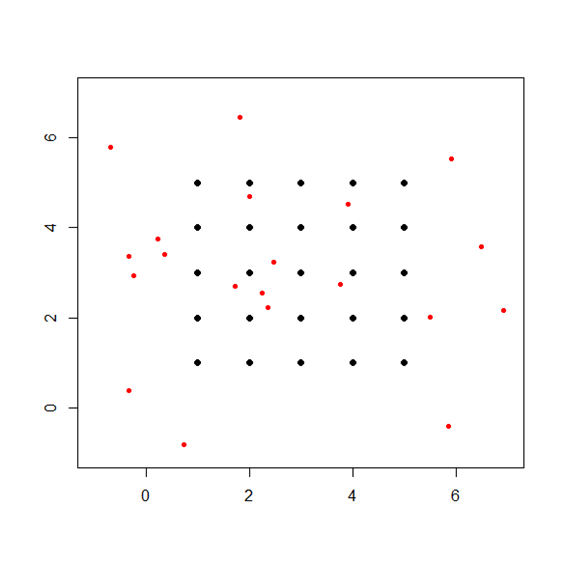
\includegraphics[height=2.5in]{Ch4/figs/binomialpoint}
\end{center}
\caption{Realization (small dots) of a binomial point process with $N=20$. The
  large dots represent trap locations.}
\label{scr0.fig.bpp}
\end{figure}

It is natural to consider a binomial point process in the context of
capture-recapture models because it preserves $N$ in the model and thus
preserves the linkage directly with closed population models. In fact,
under the binomial point process model, model $M_0$ and other closed
models are simple limiting cases of SCR models, i.e., as the
coefficient on distance ($\alpha_1$ above) tends to 0.
In addition, use of
the BPP model allows us to use data augmentation for Bayesian analysis
of the models as in Chapt. \ref{chapt.closed}, thus yielding a methodologically
coherent approach to analyzing the different classes of
models. Despite this, making explicit assumptions about $N$, such as
Poisson, is convenient in some cases (see Chapt. \ref{chapt.hscr}).

One consequence of having fixed $N$, in the BPP model, is that the
model is not strictly a model of ``complete spatial randomness''. This
is because if one forms counts $n(A_{1}),\ldots, n(A_{k})$ in any set
of disjoint regions say $A_{1}, \ldots, A_{k}$, then these counts are
{\it not} independent.  In fact, they have a multinomial distribution
\citep[see][p. 61]{illian_etal:2008}. Thus, the BPP model introduces
a slight bit of dependence in the distribution of points. However, in
most situations this will have no practical effect on any inference or
analysis and, as a practical matter, we will usually regard the BPP
model as one of spatial independence among individual activity centers
because each activity center is distributed independently of each
other activity center. Despite this implicit independence we see in
Fig. \ref{scr0.fig.bpp} that {\it realizations} of randomly distributed
points will typically exhibit distinct non-uniformity. Thus,
independent, uniformly distributed points will almost never appear
regularly, uniformly or systematically distributed. For this reason,
the basic binomial (or Poisson) point process models are enormously
useful in practical settings.  More relevant for SCR models is that we
actually have a little bit of data for some individuals and thus the
resulting posterior point pattern can deviate strongly from
uniformity, a point we come back to repeatedly in this book.
The uniformity hypothesis is only
a {\it prior} distribution which is directly affected by the quantity
and quality of the observed data, to produce a posterior distribution which
may appear distinctly non-uniform.


\subsection{The state-space of the point process}

Shortly we will focus on Bayesian analysis of this model with $N$
known so that we can directly apply to this situation what we learned
in Chapt. \ref{chapt.glms}. To do this, we note that the individual
effects ${\bf s}_{i},\ldots, {\bf s}_{N}$ are unknown quantities and
we will need to be able to simulate each ${\bf s}_{i}$ in the
population from the posterior distribution.  It should be self-evident
that we cannot simulate the ${\bf s}_{i}$ unless we describe precisely
the region over which they are uniformly distributed. This is the
quantity referred to above as the state-space, denoted henceforth by
${\cal S}$, which is a region or a set of points comprising the
potential values of ${\bf s}_{i}$. Thus, an equivalent explicit
statement of the ``uniformity assumption'' is
\[
{\bf s}_{i} \sim \mbox{Unif}({\cal S})
\]
where ${\cal S}$ is a precisely defined region. e.g., in Fig. 
\ref{scr0.fig.bpp}, ${\cal S}$ is the square defined by $[-1,7] \times
[-1, 7]$. Thus each of the $N=20$ points were generated by randomly
selecting each coordinate on the line $[-1, 7]$. 


\subsubsection{Prescribing the state-space}

Evidently, we need to define the state-space, ${\cal S}$. How can we
possibly do this objectively? Prescribing any particular ${\cal S}$
seems like the equivalent of specifying a ``buffer'' which we
criticized previously as being ad hoc. How is it, then, that the
choice of a state-space is {\it not} ad hoc? As a practical matter, it
turns out that estimates of density are insensitive to choice of the
state-space. As we observed in Chapt. \ref{chapt.closed}, it is true
that $N$ increases with ${\cal S}$, but only at the same rate as the
area of ${\cal S}$ increases under the prior assumption of constant
density. As a result, we say that density is invariant to ${\cal S}$
as long as ${\cal S}$ is sufficiently large. Thus, while choice of
${\cal S}$ is (or can be) essentially arbitrary, once ${\cal S}$ is
chosen, it defines the population being exposed to sampling, which
scales appropriately with the size of the state-space.

For our simulated system developed previously in this chapter, we
defined the state-space to be a square within which our trap array was
centered. For many practical situations this might be an
acceptable approach to defining the state-space. We provide an example
of this in sec. \ref{scr0.sec.wolverine} below in which the trap array is
irregular and also situated within a realistic landscape that is
distinctly irregular.  In general, it is most practical to define the
state-space as a regular polygon (e.g., rectangle) containing the trap
array without differentiating unsuitable habitat. Although defining
the state-space to be a regular polygon has computational advantages
(e.g., we can implement this more efficiently in {\bf WinBUGS} and
cannot for irregular polygons), a regular polygon induces an apparent
problem of admitting into the state-space regions that are distinctly
non-habitat (e.g., oceans, large lakes, ice fields, etc.).  It is
difficult to describe complex sets in mathematical terms that can be
used in {\bf BUGS}. As an alternative, we can provide a
representation of the state-space as a discrete set of points (sec.
\ref{scr0.sec.discrete}), that will allow specific points to be deleted
or not depending on whether they represent habitat, or we can define
the state-space as an arbitrary  collection of polygons stored as a GIS
shapefile
which can be analyzed easily using MCMC
(see sec. \ref{mcmc.sec.state-space}), but not so easily in the {\bf
  BUGS} variants.  In what follows below we provide an
analysis of the camera data defining the state-space to be a regular
continuous polygon (a rectangle).


\subsection{Invariance and the state-space as a model assumption}
\label{scr0.sec.invariance}

We will assert for all models we consider in this book that density is
invariant to the size and extent of ${\cal S}$, if ${\cal S}$ is
sufficiently large, and as long as our model relating $p_{ij}$ to
${\bf s}_{i}$ is a decreasing function of distance.  We can prove this
easily by drawing an analogy with a 1-d case involving distance
sampling.  Let $y_{j}$ be the number of individuals captured in some
interval $[d_{j-1},d_{j})$, and define $d_{J} = B$ for some large
value of $B$.  The observations from a survey are $y_{1},\ldots,y_J$
and the likelihood is a multinomial likelihood, so the log-likelihood
is of the form
\[
\mbox{logL}(\{ y_{j} \}) = \sum_{j=1}^{J} y_{j} \log( \pi_{j} )
\]
where $\pi_{j}$ is the probability of detecting an individual in
distance class $j$, which depends on parameters of the detection
function (the manner of which is not relevant for the present
discussion).  For $B$ sufficiently large, we guarantee that $E(y_{J})
= 0$ and therefore the observed frequency in the ``last cell''
contributes nothing to the likelihood, in regular situations in which
the detection function decays monotonically with distance and prior
density is constant.


Sometimes our estimate of density can be affected by choosing ${\cal
  S}$ too small. However, this might be sensible if ${\cal S}$ is
naturally well-defined. As we discussed in Chapt. \ref{chapt.intro},
{\bf choice of ${\cal S}$ is part of the model}, and thus it is
sensible that estimates of density might be sensitive to its
definition in problems where it is natural to restrict ${\cal S}$.
One could imagine, however, that in specific cases where you're
studying a small population with well-defined habitat preferences,
that a problem could arise because changing the state-space around
based on differing opinions and GIS layers might have substantial
changes on the density estimates and hence those of population
size. But this is a real biological problem and a natural consequence
of the spatial formalization of capture-recapture models - a feature,
not a bug or some statistical artifact - and it should be resolved
with better information, research, and thinking.  For situations where
there is not a natural choice of ${\cal S}$, we should default to
choosing ${\cal S}$ to be very large in order to achieve invariance
or, otherwise, evaluate sensitivity of density estimates by trying a
couple of different choices of ${\cal S}$. This is a standard
``sensitivity to prior'' argument that Bayesians always have to be
conscious of.  We demonstrate this in our analysis of section
\ref{scr0.sec.wolverine} below. As an additional practical
consideration, we note that $area({\cal S})$ affects data
augmentation. If you increase $area({\cal S})$ then there are more
individuals to account for and therefore the size of the augmented
data set $M$ must increase.

We have been told that one can carry-out non-Bayesian analyses of SCR
models without having to specify the state-space of the point process
or perhaps while only specifying it imprecisely.  This assertion is
incorrect. We assume people are thinking this because {\it they} don't
have to specify it explicitly because someone else has done it for
them in a convenient software package, e.g., perhaps that does
likelihood analysis. Even to do
integrated likelihood (see Chapt. \ref{chapt.mle}) we have to integrate the
conditional-on-${\bf s}$ likelihood over some 2-dimensional space.  It might
work that the integration can be done from $-\infty$ to $+\infty$ but
that is a mathematical artifact of specific detection functions, and
not a general feature. Moreover, this amounts to 
an implicit definition of a state-space that doesn't make biological
sense in any real context. %%%, even though it may in fact be innocuous.


\subsection{Connection to Model  $M_h$}  \label{scr0.sec.scrmh}

SCR models are closely related to heterogeneity models. In SCR models,
heterogeneity in encounter probability is induced by both the effect
of distance in the model for detection probability and also from
specification of the state-space. Hence, the state-space  is an
explicit element of the model. 
To understand this, suppose we have a random
effect with some prior distribution:
\[
{\bf s} \sim \mbox{Unif}({\cal S})
\]
and encounter probability is a function of ${\bf s}$, denoted by 
 $p({\bf s}) = p(y=1|{\bf s})$. 
For example, under Eq. \ref{scr0.eq.logit}
we have that 
\[
p({\bf s}) = logit^{-1} ( \alpha_{0} + \alpha_1 ||{\bf
  s}_{i}-{\bf x}_{j} || )
\]
and we can work out, either analytically or empirically, what is the
implied distribution of $p$ for a population of individuals.  We show
an illustration in Fig. \ref{scr0.fig.buffereffect} which shows a
histogram of $p$ for a hypothetical population of 100000 individuals
on a state-space enclosing our $5 \times 5$ trap array above, under
the logistic model for distance given by Eq. \ref{scr0.eq.logit}. {\bf
  R} code is provided in the {\bf R} package \mbox{\tt scrbook} to
produce this analysis for the logistic and half-normal models. The
histogram shows the encounter probability under buffers of 0.2, 0.5
and 1.0. We see the mass shifts to the left as the buffer increases,
implying more individuals with lower encounter probabilities, as their
home range centers increase in distance from the trap array.


\begin{figure}
\begin{center}
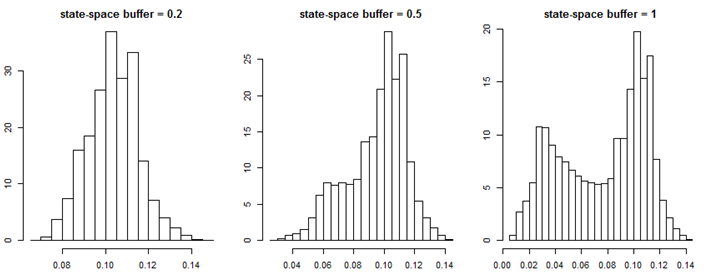
\includegraphics[width=5in]{Ch4/figs/buffereffect}
\end{center}
\caption{Implied population distribution of $p_{i}$ for a population
  of individuals as a function of the size of the state-space buffer
  around a trap array. The trap array is fixed and centered within a
  square state-space.
xxxxxxxxxxxxxxx
The main titles of the three panel plots are too small. I would rather
call them (a), (b) and (c) and then give their associated information
in the figure legend. Also, numbers on axes are very small for the
sight of men in our age  xxxxxxxxxxxxxxxxxxxx
}
\label{scr0.fig.buffereffect}
\end{figure}

Another way to understand this is by representing ${\cal S}$ as a set
of discrete points on a grid. In the coarsest possible case where
${\cal S}$ is a single arbitrary point, then every individual has
exactly the same $p$. As we increase the number of points in ${\cal
  S}$,  more distinct values of $p$ are possible. As such, when
${\cal S}$ is characterized by discrete points then SCR models are
precisely a type of finite-mixture model \citep{norris_pollock:1996,
  pledger:2000}, except, in the case of SCR models, we have some information about which
group an individual belong (i.e., where their activity center is), as
a result of their captures in traps.

This context suggests the problem raised by \citet{link:2003}. He
showed that in most practical situations $N$ may not be identifiable
across classes of mixture distributions which in the context of SCR
models is the pair $(g, {\cal S})$.  The difference, however, is that
we do obtain some direct information about ${\bf s}$ in SCR models and
therefore it may be reasonable to expect that
$N$ is identifiable across models characterized by $(g,{\cal
  S})$.

\subsection{Connection to Distance Sampling}

It is worth re-emphasizing that the basic SCR model is a binomial
encounter model in which distance is a covariate. As such, it is
strikingly similar to a classical distance sampling model
\citep{buckland_etal:2002}. Both have distance as a covariate but in
classical distance sampling problems the focus is on the distance
between the observer and the animal at an instant in time, not the
distance between a trap and an animal's home range center. As a
practical matter, in distance sampling, ``distance'' is {\it observed}
for those individuals that appear in the sample. Conversely, in SCR
problems, it is only imperfectly observed (we have partial information
in the form of trap observations).  Clearly, it is preferable to
observe distance if possible, but distance sampling requires field
methods that are often not practical in many situations, e.g. when
studying carnivores such as bears or large cats. Furthermore, SCR
models allow us to relax many of the assumptions made in classical
distance sampling, such as perfect detection at distance zero, and SCR
models allow for estimates of quantities other than density, such as
home range size, and space usage (see Chapts. \ref{chapt.rsf} and
\ref{chapt.ecoldist}).


\section{Simulating SCR Data}

It is always useful to simulate data because it allows you to
understand the system that you're modeling and also calibrate your
understanding with the parameter values of the model. That is, you can
simulate data using different parameter values until you obtain data
that ``look right'' based on your knowledge of the specific situation
that you're interested in. Here we provide a simple script to
illustrate how to simulate spatial encounter history data. In this
exercise we simulate data for 100 individuals and a 25 trap array laid
out in a $5 \times 5$ grid of unit spacing.  The specific encounter
model is the half-normal model given above and we used this code to
simulate data used in subsequent analyses.  The 100 activity centers
were simulated on a state-space defined by a $8 \times 8$ square
within which the trap array was centered (thus the trap array is
buffered by 2 units). Therefore, the density of individuals in this
system is fixed at $100/64$.

{\small
\begin{verbatim}
	set.seed(2013)
# create 5 x 5 grid of trap locations with unit spacing
traplocs<- cbind(sort(rep(1:5,5)),rep(1:5,5))
Dmat<-e2dist(traplocs,traplocs) 
ntraps<-nrow(traplocs)

# define state-space of point process. (i.e., where animals live).
# "delta" just adds a fixed buffer to the outer extent of the traps.
delta<-2
Xl<-min(traplocs[,1] - delta)
Xu<-max(traplocs[,1] + delta)
Yl<-min(traplocs[,2] - delta)
Yu<-max(traplocs[,2] + delta)

N<-100   # population size
K<- 20    # number nights of effort

sx<-runif(N,Xl,Xu)    # simulate activity centers
sy<-runif(N,Yl,Yu)
S<-cbind(sx,sy)
D<- e2dist(S,traplocs)  # distance of each individual from each trap

alpha0<- -2.5      # define parameters of encounter probability
sigma<- 0.5        # scale parameter of half-normal
alpha1<- 1/(2*sigma*sigma) # convert to coefficient on distance

probcap<- plogis(-2.5)*exp( - alpha1*D*D)    # probability of encounter 
# now generate the encounters of every individual in every trap
Y<-matrix(NA,nrow=N,ncol=ntraps)
for(i in 1:nrow(Y)){
   Y[i,]<-rbinom(ntraps,K,probcap[i,])
}
\end{verbatim}
}

We remind the reader that, in presenting \R or other code snippets
throughout the book, we will deviate from our standard variable
expressions for some quantities. 
In particular, we sometimes 
substitute words for integer variable designations:
\mbox{\tt nind} (for $n$), \mbox{\tt ntraps} (for $J$), and \mbox{\tt
 nperiods} (for $K$). In our opinion this leaves less to be infereed
 in a \bugs model definition.

 Subsequently we will generate data using this code packaged in an
 {\bf R} function called \mbox{\tt simSCR0.fn} in the package
 \mbox{\tt scrbook} which takes a number of arguments including
 \mbox{\tt discard0} which, if \mbox{\tt TRUE}, will return only the
 encounter histories for captured individuals.  A second argument is
 \mbox{\tt array3d} which, if \mbox{\tt TRUE}, returns the 3-d
 encounter history array instead of the aggregated \mbox{\tt nind}
 $\times \mbox{\tt ntraps}$ encounter frequencies (see below). Finally
 we provide a random number seed, \mbox{\tt sd = 2013} to ensure
 repeatability of the analysis here. We obtain a data set as above
 using the following command:
\begin{verbatim}
data<-simSCR0.fn(discard0=TRUE,array3d=FALSE,sd=2013)
\end{verbatim}
The {\bf R} object \mbox{\tt data} is a list, so let's take a look at
what's in the list and then harvest some of its elements for further
analysis below.
{\small
\begin{verbatim}
> names(data)
[1] "Y"        "traplocs" "xlim"     "ylim"     "N"        "alpha0"   "beta"
[8] "sigma"    "K"

> Y<-data$Y
> traplocs<-data$traplocs
\end{verbatim}
}

\subsection{Formatting and manipulating real data sets}
\label{scr0.sec.formats}

Conventional capture-recapture data are easily stored and manipulated
as a 2-dimensional array, an $\mbox{\tt nind} \times \mbox{\tt
  nperiods}$ matrix, which is maximally informative for any
conventional capture-recapture model, but not for spatial
capture-recapture models.  For SCR models we must preserve the spatial
information in the encounter history information. We will routinely
analyze data from 3 standard formats:
\begin{itemize}
\item[(1)] The basic 2-dimensional data format, which is an \mbox{\tt
    nind} $\times$ \mbox{\tt ntraps} encounter frequency matrix such
  as that simulated previously. These are the total number of encounters in each
  trap, summed over replicate samples.
\item[(2)] The maximally informative 3-dimensional array, for which we
  establish here the convention that it has dimensions \mbox{\tt nind}
  $\times$ \mbox{\tt nperiods} $\times$ \mbox{\tt ntraps}.
\item[(3)] We use a compact format - the ``SCR flat format'' - which
  we describe below in section \ref{scr0.sec.wolverine}.
\end{itemize}
To simulate data in the most informative format - the ``3-d array'' -
we can use the {\bf R} commands given previously but replace the last
4 lines with the following:
{\small
\begin{verbatim}
Y<-array(NA,dim=c(N,K,ntraps))
for(i in 1:nrow(Y)){
for(j in 1:ntraps){
 Y[i,1:K,j]<-rbinom(K,1,probcap[i,j])
}
}
\end{verbatim}
} 

We see that a collection of $K$ binary encounter events are
generated for {\it each} individual and for {\it each} trap.  The
probabilities of those Bernoulli trials are computed based on the
distance from each individuals home range center and the trap (see
calculation above), and those are housed in the matrix \mbox{\tt
  probcap}. Our data simulator function \mbox{\tt simSRC0.fn} will
return the full 3-d array if \mbox{\tt array3d=TRUE} is specified in
the function call.  To recover the 2-d matrix from the 3-d array, and
subset the 3-d array to individuals that were captured, we do this:
{\small
\begin{verbatim}
Y2d<- apply(Y,c(1,3),sum) # sum over the ``replicates'' dimension (2nd margin of the array)
ncaps<-apply(Y2d,1,sum)   # compute how many times each individual was captured
Y<-Y[ncaps>0,,]           # keep those individuals that were captured
\end{verbatim}
}

\section{Fitting an SCR Model in BUGS}
\label{scr0.sec.winbugs1}

Clearly if we somehow knew the value of $N$ then we could fit this
model directly because, in that case, it is a special kind of logistic
regression model - one with a random effect, but that enters into the
model in a peculiar fashion - and also with a distribution (uniform)
which we don't usually think of as standard for random effects models.
So our aim here is to analyze the known-$N$ problem, using our
simulated data, as an incremental step in our progress toward fitting
more generally useful models.

To begin, we use our simulator to grab a data set and then harvest the
elements of the resulting object for further analysis.
\begin{verbatim}
data<-simSCR0.fn(discard0=FALSE,sd=2013)
y<-data$Y
traplocs<-data$traplocs
nind<-nrow(y)
X<-data$traplocs
J<-nrow(X)
y<-rbind(y,matrix(0,nrow=(100-nrow(y)),ncol=J ) )
Xl<-data$xlim[1]
Yl<-data$ylim[1]
Xu<-data$xlim[2]
Yu<-data$ylim[2]
\end{verbatim}

Note that we specify \mbox{\tt discard0 = FALSE} so that we have a
"complete" data set, i.e., one with the all-zero encounter histories
corresponding to uncaptured individuals. Now, within an {\bf R} session, we
can create the {\bf BUGS} model file and fit the model using the following
commands.  {\bf XXXX Note: run model with "sigma" as below XXXXXX}
{\small
\begin{verbatim}
cat("
model {
alpha0~dnorm(0,.1)
logit(p0)<- alpha0
alpha1~dnorm(0,.1)
sigma<- sqrt(1/(2*alpha1))
for(i in 1:N){  # note N here because N is KNOWN in this example
   s[i,1]~dunif(Xl,Xu)
   s[i,2]~dunif(Yl,Yu)    
for(j in 1:J){
d[i,j]<- pow(pow(s[i,1]-X[j,1],2) + pow(s[i,2]-X[j,2],2),0.5)
y[i,j] ~ dbin(p[i,j],K)
p[i,j]<- p0*exp(- alpha1*d[i,j]*d[i,j])
}
}

}
",file = "SCR0a.txt")
\end{verbatim}
}
This model describes the half-normal detection model but it
would be trivial to modify that to various others including the
logistic described above. One consequence of using the half-normal is
that we have to constrain the encounter probability to be in $[0,1]$
which we do here by defining \mbox{\tt alpha0} to be the logit of the
intercept parameter \mbox{\tt p0}. Note that the distance covariate is
computed within the {\bf BUGS} model specification given the matrix of trap
locations, \mbox{\tt X}, which is provided to {\bf WinBUGS} as data.

Next we do a number of organizational activities including bundling
the data for {\bf WinBUGS}, defining some initial values, the parameters to
monitor and some basic MCMC settings.  We choose initial values for
the activity centers ${\bf s}$ by generating uniform random numbers in
the state-space but, for the observed individuals, we replace those
values by each individual's mean trap coordinate for all encounters
{\small
\begin{verbatim}
sst<-cbind(runif(nind,Xl,Xu),runif(nind,Yl,Yu))  # starting values for s
for(i in 1:nind){
if(sum(y[i,])==0) next
sst[i,1]<- mean( X[y[i,]>0,1] )
sst[i,2]<- mean( X[y[i,]>0,2] )
}

data <- list (y=y,X=X,K=K,N=nind,J=J,Xl=Xl,Yl=Yl,Xu=Xu,Yu=Yu)
inits <- function(){
  list (alpha0=rnorm(1,-4,.4),alpha1=runif(1,1,2),s=sst)
}

library("R2WinBUGS")
parameters <- c("alpha0","alpha1","sigma")
nthin<-1
nc<-3
nb<-1000
ni<-2000
out <- bugs (data, inits, parameters, "SCR0a.txt", n.thin=nthin, n.chains=nc, 
         n.burnin=nb,n.iter=ni,debug=TRUE,working.dir=getwd())
\end{verbatim}
}
There is little to say about the preceding operations other than
to suggest that you might explore the output and investigate 
additional analyses by running the \mbox{\tt simSCR0.fn} script provided in the {\bf R}
package \mbox{\tt scrbook}. 

For purposes here, we ran $1000$ burn-in and $1000$ post-burn-in
iterations, and 3 chains,
to obtain 3000 posterior samples.  Because we know $N$ for this
particular data set we only have 2 parameters of the detection model
to summarize (\mbox{\tt alpha0} and \mbox{\tt alpha1}), along with the
derived parameter $\sigma$, the scale parameter of the Gaussian
kernel, i.e., $\sigma = \sqrt{1/(2\alpha_{1})}$.  When the
object \mbox{\tt out} is produced we print a summary of the results as
follows:
{\small
\begin{verbatim}
> print(out,digits=3)
Inference for Bugs model at "SCR0a.txt", fit using WinBUGS,
 3 chains, each with 2000 iterations (first 1000 discarded)
 n.sims = 3000 iterations saved
            mean     sd    2.5%     25%    50%     75%   97.5%  Rhat n.eff
alpha0    -2.496  0.224  -2.954  -2.648  -2.48  -2.340  -2.091 1.013   190
alpha1     2.442  0.419   1.638   2.145   2.44   2.721   3.303 1.005   530
sigma      NEED RESULTS WITH SIGMA HERE .....
deviance 292.803 21.155 255.597 277.500 291.90 306.000 339.302 1.006   380
.
 [some output deleted]
.
\end{verbatim}
}
We know the data were generated with \mbox{\tt alpha0} $= -2.5$ and
\mbox{\tt alpha1 = -2}. The estimates look reasonably close to those
data-generating values and we probably feel pretty good about the
performance of the Bayesian analysis and MCMC algorithm that {\bf WinBUGS}
cooked-up based on our sample size of 1 data set.  It is worth noting
that the Rhat statistics indicate reasonable convergence but, as a
practical matter, we might choose to run the MCMC algorithm for
additional time to bring these closer to 1.0 and to increase the
effective posterior sample size (\mbox{\tt n.eff}). Other summary output includes
``deviance'' and related things including the deviance information
criterion (DIC). We discuss these things in Chapts. \ref{chapt.mcmc}
and \ref{chapt.gof}.



\section{Unknown N}
\label{scr0.sec.unknownN}

In all real applications $N$ is unknown.
 We handled this
important issue in Chapt. \ref{chapt.closed} using the method of data augmentation
which we apply here to achieve a realistic analysis of model SCR0. As
with the basic closed population models considered previously, we
formulate the problem here by augmenting our observed data set with a
number of ``all-zero'' encounter histories - what we referred to in
Chapt. \ref{chapt.closed} as potential individuals. If $n$ is the number of observed
individuals, then let $M-n$ be the number of potential individuals in
the data set. For the basic $y_{ij}$ data structure (individuals x
traps encounter frequencies) we simply add additional rows of all-zero
observations to that data set. This is because such
``individuals'' are unobserved, and therefore necessarily have
$y_{ij}=0$ for all $j$.  A data set, say with 4 traps and 6 individuals,
augmented with 4 pseudo-individuals therefore might look like this:
{\small
\begin{verbatim}
      trap1 trap2 trap3 trap4
 [1,]     1     0     0     0
 [2,]     0     2     0     0
 [3,]     0     0     0     1
 [4,]     0     1     0     0
 [5,]     0     0     1     1
 [6,]     1     0     1     0
 [7,]     0     0     0     0
 [8,]     0     0     0     0
 [9,]     0     0     0     0
[10,]     0     0     0     0
\end{verbatim}
}
We typically have more than 4 traps and, if we're fortunate, many more
individuals in our data set.

For the augmented data, we introduce a set of binary latent variables
(the data augmentation variables), $z_{i}$, and the model is extended
to describe $\Pr(z_{i} = 1)$ which is, in the context of this problem,
the probability that an individual in the augmented data set is a
member of the population that was sampled. In other words, if $z_{i}=1$
for one of the all-zero encounter histories, this is implied to be
a sampling zero whereas observations for which $z_{i}=0$ are
``structural zeros'' under the model.

How big does the augmented data set have to be? We discussed this
issue in Chapt. \ref{chapt.closed} where we noted that the size of the
data set is equivalent to the upper limit of a uniform prior
distribution on $N$.  Practically speaking, it should be sufficiently
large so that the posterior distribution for $N$ is not truncated. On
the other hand, if it is too large then unnecessary calculations are
being done. An approach to choosing $M$ by trial-and-error is
indicated. You can take a ballpark estimate of the probability that an
individual is captured at all during the study, say $\tilde{p}$, which
is related to the ``per sample'' encounter probability, $p$, by
$\tilde{p} = 1-(1-p)^{K}$, obtain $N$ as $n/\tilde{p}$, and then set
$M = 2*N$, as a first guess. Do a short MCMC run and then consider
whether you need to increase $M$. See Chapt. \ref{chapt.mcmc} for an
example of this. \citet[][ch. 6]{kery_schaub:2011} provide an
assessment of choosing $M$ in closed population models.

Analysis by data augmentation removes $N$ as an explicit parameter of
the model. Instead, $N$ is a derived parameter, computed by $N=
\sum_{i=1}^{M} z_{i}$. Similarly, {\it density}, $D$, is also a
derived parameter computed as $D=N/area({\cal S})$. For our
simulator, we're using an $8 \times 8$ state-space and thus we will
compute $D$ as $D=N/64$.

\subsection{Analysis using data augmentation in WinBUGS}

As before we begin by obtaining a data set using our \mbox{\tt
  simSCR0.fn} routine and then harvesting the required data objects
from the resulting data list.  Note that we use the \mbox{\tt
  discard0=TRUE} option this time so that we get a ``real looking'' data set
with no all-zero encounter histories. After harvesting the data we
produce the {\bf WinBUGS} model specification which now includes $M$
encounter histories including the augmented potential individuals, the
data augmentation parameters $z_{i}$, and the data augmentation
parameter $\psi$. {\bf XXX Need to re-run with sigma inserted XXXX}
{\small
\begin{verbatim}
data<-simSCR0.fn(discard0=TRUE,sd=2013)
y<-data$Y
traplocs<-data$traplocs
nind<-nrow(y)
X<-data$traplocs
J<-nrow(X)
Xl<-data$xlim[1]
Yl<-data$ylim[1]
Xu<-data$xlim[2]
Yu<-data$ylim[2]

cat("
model {
alpha0~dnorm(0,.1)
logit(p0)<- alpha0
alpha1~dnorm(0,.1)
sigma<- sqrt(1/(2*alpha1))
psi~dunif(0,1)

for(i in 1:M){    
   z[i] ~ dbern(psi)
   s[i,1]~dunif(Xl,Xu)
   s[i,2]~dunif(Yl,Yu)
   for(j in 1:J){
      d[i,j]<- pow(pow(s[i,1]-X[j,1],2) + pow(s[i,2]-X[j,2],2),0.5)
      y[i,j] ~ dbin(p[i,j],K)
      p[i,j]<- z[i]*p0*exp(- alpha1*d[i,j]*d[i,j])
   }
}
N<-sum(z[])
D<-N/64
}
",file = "SCR0a.txt")
\end{verbatim}
}

To prepare our data we have to augment the data matrix \mbox{\tt y}
with $M-n$ all-zero encounter histories, we have to create starting
values for the variables $z_{i}$ and also the activity centers ${\bf
  s}_{i}$ of which, for each, we require $M$ values. Otherwise the
remainder of the code for bundling the data, creating initial values
and executing {\bf WinBUGS} looks much the same as before except with more
or differently named arguments.
{\small
\begin{verbatim}
## Data augmentation stuff
M<-200
y<-rbind(y,matrix(0,nrow=M-nind,ncol=ncol(y)))
z<-c(rep(1,nind),rep(0,M-nind))

sst<-cbind(runif(M,Xl,Xu),runif(M,Yl,Yu))  # starting values for s
for(i in 1:nind){
   if(sum(y[i,])==0) next
   sst[i,1]<- mean( X[y[i,]>0,1] )
   sst[i,2]<- mean( X[y[i,]>0,2] )
}
data <- list (y=y,X=X,K=K,M=M,J=J,Xl=Xl,Yl=Yl,Xu=Xu,Yu=Yu)
inits <- function(){
  list (alpha0=rnorm(1,-4,.4),alpha1=runif(1,1,2),s=sst,z=z)
}

library("R2WinBUGS")
parameters <- c("alpha0","alpha1","sigma","N")
nthin<-1
nc<-3
nb<-1000
ni<-2000
out <- bugs (data, inits, parameters, "SCR0a.txt", n.thin=nthin,n.chains=nc,
 n.burnin=nb,n.iter=ni,debug=TRUE,working.dir=getwd())
\end{verbatim}
}

{\bf Remarks}:  (1) Note the differences in this new {\bf WinBUGS} model
with that appearing in the known-$N$ version.  (2) Also the input data
has changed - the augmented data set has more rows of
all-zero encounter histories. Previously we knew that $N=100$ but in this analysis we
pretend not to know $N$, but think that $N=200$ is a good upper bound;
(3) Population size $N({\cal S})$ is a derived parameter, being computed by
summing up all of the data augmentation variables $z_{i}$ (as we've
done previously in Chapt. \ref{chapt.closed}); (4) Density, $D\equiv D({\cal S})$, is also a derived
parameter. Summarizing the output from {\bf WinBUGS} produces:
{\small
\begin{verbatim}
> print(out1,digits=2)
Inference for Bugs model at "SCR0a.txt", fit using WinBUGS,
 3 chains, each with 2000 iterations (first 1000 discarded)
 n.sims = 3000 iterations saved
           mean    sd   2.5%    25%    50%    75%  97.5% Rhat n.eff
alpha0    -2.57  0.23  -3.04  -2.72  -2.56  -2.41  -2.15 1.01   320
alpha1     2.46  0.42   1.63   2.16   2.46   2.73   3.33 1.02   120
N        113.62 15.73  86.00 102.00 113.00 124.00 147.00 1.01   260
D          1.78  0.25   1.34   1.59   1.77   1.94   2.30 1.01   260
sigma      0.46  0.04   0.39   0.43   0.45   0.48   0.55 1.02   120
deviance 302.60 23.67 261.19 285.47 301.50 317.90 354.91 1.00  1400

For each parameter, n.eff is a crude measure of effective sample size,
and Rhat is the potential scale reduction factor (at convergence, Rhat=1).

DIC info (using the rule, pD = var(deviance)/2)
pD = 279.9 and DIC = 582.5
DIC is an estimate of expected predictive error (lower deviance is better).
\end{verbatim}
}
\begin{comment}
The column labeled ``MC error'' (see sec. \ref{glms.sec.convergence})
XXXXX this is only shown in WinBUGS?
own log file, but not in the above table produced by
R2WinBUGS XXXX. Apparently, this is what ?Time-series SE? and ?Naive SE? in
the output from ?rjags? by JAGS means, but I never understood this
before XXXXXX XXXX is this out of place? Where is first occurrence of
WinBUGS output XXXXXXXXX  
is the Monte Carlo error - the error
inherent in the attempt to compute these posterior summaries by
MCMC
(see secs.  for discussion of this quantity
\ref{glms.sec.convergence} \ref{mcmc.sec.mcmcsummary}).
It is desirable to run the Markov chain algorithm long enough so
as to reduce the MC error to a tolerable level. What constitutes
tolerable is up to the investigator. Certainly less than 1\% is called
for. 
\end{comment}
The Rhat statistic (discussed in secs. \ref{glms.sec.convergence} and
\ref{mcmc.sec.mcmcsummary}) for this analysis indicates satisfactory
convergence. 
%As a general rule, Rhat gets closer to 1 (and Monte Carlo error decreases)
%as the number of iterations increases.  
We see that the
estimated parameters ($\alpha_0$ and $\alpha_1$) are comparable to the
previous results obtained for the known-$N$ case, and also not too
different from the data-generating values. The posterior of $N$
overlaps the data-generating value substantially.

We note that these results were obtained from a fit of the actual
data-generating model, i.e., that based on the half-normal detection
model, to a single simulated data set. Sometimes it is useful to
investigate how various {\it wrong} models perform.  Therefore, for
fun and excitement, we fit the logistic-linear detection model
(Eq. \ref{scr0.eq.logit}), to the same data set. This is easily
achieved by modifying the {\bf WinBUGS} model specification above,
although we provide the {\bf R} script \mbox{\tt SCR0bayes} in the
{\bf R} package \mbox{\tt scrbook}.  Those results are given below. We
see that the estimate of $N$, the main parameter of interest, is not
too dissimilar from that obtained under the correct model, convergence
is worse (as measured by Rhat) which may not have anything to do with
the model being wrong, and the posterior deviance favors the correct
model (it is smaller) while, interestingly, the DIC does not.  We
consider the effectiveness of DIC for carrying-out model selection in
Chapt.  \ref{chapt.gof}.  
{\small
\begin{verbatim}
Inference for Bugs model at "SCR0a.txt", fit using WinBUGS,
 3 chains, each with 2000 iterations (first 1000 discarded)
 n.sims = 3000 iterations saved
           mean    sd   2.5%    25%    50%    75%  97.5% Rhat n.eff
alpha0    -0.47  0.17  -0.80  -0.58  -0.48  -0.36  -0.11 1.05    49
alpha1     3.86  0.44   3.08   3.56   3.82   4.15   4.87 1.03    84
N        118.29 19.15  86.00 105.00 117.00 129.00 163.00 1.01   270
D          1.85  0.30   1.34   1.64   1.83   2.02   2.55 1.01   270
deviance 310.44 22.85 268.50 294.50 310.00 324.90 358.50 1.02   100

For each parameter, n.eff is a crude measure of effective sample size,
and Rhat is the potential scale reduction factor (at convergence, Rhat=1).

DIC info (using the rule, pD = var(deviance)/2)
pD = 256.0 and DIC = 566.4
DIC is an estimate of expected predictive error (lower deviance is better).
\end{verbatim}
}


\subsection{Implied Home Range Area}

Here we apply the method described in sec. \ref{scr0.sec.implied} to
compute the effective home range area under some different encounter
probability models fit to simulated data. 
We simulated data from the Gaussian kernel model as in 
sec. \ref{scr0.sec.unknownN} and then we fitted 4 models to it: (1)
the true data-generating model; (2) the ``hazard'' or complementary log-log link 
model (Eq. \ref{scr0.eq.hazard}); (3) the negative exponential model
and (4) the logit model (Eq. \ref{scr0.eq.logit}).
We modified the function \mbox{\tt  SCR0bayes} for this purpose which
you should be able to do with little difficulty. We fit each model to
the same simulated  data set using \winbugs, based only on 1000
post-burn-in samples and 3 chains, which produced the posterior
summaries given in Tab. \ref{scr0.tab.implied}.

XXXXXXXXXXXXXXXXX
We could use the MCMC histories of parameters to compute the posterior
mean of the ehra too.....
XXXXXXXXXXXXXXXXXXXX
Comment: wow, the implied home range area can be pretty different thre
is only minor differences in estimated N.
We emphasize that sigma means a different thing under every model. 


\begin{table}
\centering
\caption{
Posterior mean of model parameters for 4 different models fitted to a
single simulated data set,
  and the effective home range area under each detection model.
}
\begin{tabular}{crrrr}
\hline \hline 
     &  Gaussian & cloglog &exponential & logit \\  \hline
$\alpha_0$  &  -2.57 &  -2.60 & -1.51 & -0.47 \\
$\alpha_1$  &  2.46  & 2.56  & 3.59  & 3.86 \\
N           & 113.62& 114.16 &119.69& 118.29 \\
D           & 1.78  & 1.78  & 1.87  & 1.85 \\
$\sigma$    & 0.46  & 0.45 &  0.28  &  -- \\
hra         & 3.85  & 3.78 &  5.51  & 2.64 \\
\end{tabular}
\label{scr0.tab.implied}
\end{table}





\subsection{Use of other BUGS engines: JAGS}

There are two other popular {\bf BUGS} engines in widespread use: {\bf
  OpenBUGS} \citep{thomas_etal:2006} and {\bf JAGS}
\citep{plummer:2003}. Both of these are easily called from {\bf
  R}. {\bf OpenBUGS} can be used instead of {\bf WinBUGS} by changing
the package option in the \mbox{\tt bugs} call to \mbox{\tt
  package=OpenBUGS}.  {\bf JAGS} can be called using the function
\mbox{\tt jags()} in package \mbox{\tt R2JAGS} which has nearly the
same arguments as \mbox{\tt bugs()}.  We prefer to use the {\bf R}
library \mbox{\tt rjags} \citep{plummer:2009} which has a slightly
different implementation that we demonstrate here as we reanalyze the
simulated data set in the previous section (note: the same {\bf R}
commands are used to generate the data and package the data, inits and
parameters to monitor). The function \mbox{\tt jags.model} is used to
initialize the model and run the MCMC algorithm for an adaptive period
during which tuning of the MCMC algorith might take place.  These
samples cannot be used for inference.  Then the Markov chains are
updated using \mbox{\tt coda.samples()} to obtain posterior samples
for analysis, as follows:
\begin{verbatim}
jm<- jags.model("SCR0a.txt", data=data, inits=inits, n.chains=nc, n.adapt=nb))
jm<- coda.samples(jm, parameters, n.iter=ni-nb, thin=nthin)
\end{verbatim}
We find that {\bf JAGS} seems to be 20-30\% faster (and often more)
for the basic SCR model which you can evaluate using the function
\mbox{\tt SCR0bayes} in the {\bf R} package \mbox{\tt
  scrbook}. \citet{hobbs:2011} provides a good introduction to
ecological modeling with {\bf JAGS} which we recommend.



\section{Wolverine Camera Trapping Study}
\label{scr0.sec.wolverine}

We provide an analysis here of camera trapping data from a study of
wolverines \emph{Gulo gulo}
\citep{magoun_etal:2011, royle_etal:2011jwm}. The study took place in
SE Alaska (Fig. \ref{scr0.fig.wolverinelocs}) where 37 cameras were
operational for variable periods of time (min = 5 days, max = 108
days, median = 45 days).  A consequence of this is that the binomial
sample size $K$ (see Eq. \ref{scr0.eq.bin}) is variable for each
camera. Thus, we must provide a matrix of sample sizes as data to {\bf
  BUGS} and modify the model specification in
sec. \ref{scr0.sec.unknownN} accordingly. Our treatment of the data
here is based on the analysis of \citet{royle_etal:2011jwm}.

\begin{figure}
\begin{center}
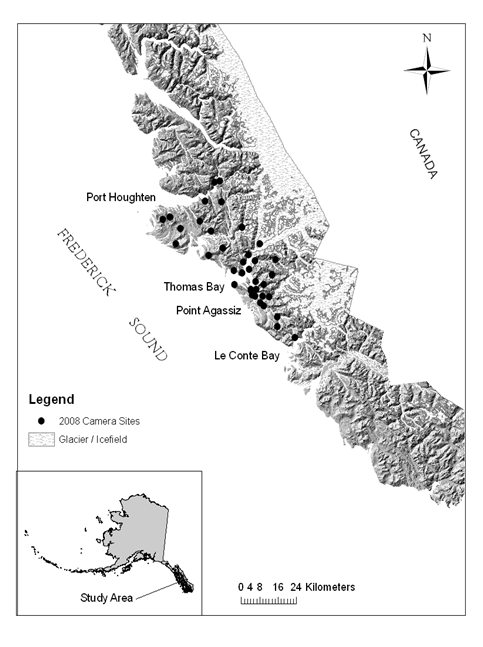
\includegraphics[height=3in]{Ch4/figs/wolverinelocs}
\end{center}
\caption{
Wolverine camera trap locations from \citet{magoun_etal:2011}.
XXXXX this figure is way too small. Also, I would take out some of the
legends in the actual figure and put this into the figure legend
(e.g., what the dots mean and the grey area) XXXXXX
}
\label{scr0.fig.wolverinelocs}
\end{figure}

To carry-out an analysis of these data, we require the matrix of trap
coordinates and the encounter history data.  We store data in the
``scr flat format'' (see sec.  \ref{scr0.sec.formats} above), an
efficient file format which is easily manipulated and also used as the
input file format in {\bf SPACECAP} \citep{gopalaswamy_etal:2012} and
in the {\bf R} package \mbox{\tt SCRbayes} \citep{russell_etal:2012}.
To illustrate this format, the wolverine data are available in the
package \mbox{\tt scrbook} by typing:
\begin{verbatim}
data(wolverine)
\end{verbatim}
which contains a list having elements \mbox{\tt wcaps} and \mbox{\tt
  wtraps}.  The ``encounter data file'' \mbox{\tt wcaps} has 3 columns
and 115 rows, each representing a unique encounter event including the
trap identity, the individual identity and the sample occasion index
(\mbox{\tt sample}).  The first 10 rows of this matrix are as follows:
{\small
\begin{verbatim}
> wolverine$wcaps[1:10,]
       trapid individual sample
  [1,]      1          2    127
  [2,]      1          2    128
  [3,]      1          2    129
  [4,]      1         18    130
  [5,]      2          3    106
  [6,]      2         18    104
  [7,]      5          5     73
  [8,]      5          5     89
  [9,]      6         18    117
 [10,]      6         18    118
\end{verbatim}
}
Each row is a unique 
individual/trap encounter, and the 3 variables (columns) are: 
\mbox{\tt trapid} -- an
integer that runs from \mbox{\tt 1:ntraps}, \mbox{\tt individual} runs from
\mbox{\tt 1:nind} and
\mbox{\tt sample} 
runs from \mbox{\tt 1:nperiods}. Often (as the case here) \mbox{\tt
  sample} 
will
correspond to daily sample intervals. The variable \mbox{\tt trapid} will have to
correspond to the row of a matrix containing the trap coordinates - in
this case the file \mbox{\tt wtraps} which we describe further below.

Note that the information provided in this encounter data file
\mbox{\tt wcaps} does not represent a completely informative summary
of the data. For example, if no individuals were captured in a certain
trap or during a certain period, then this compact data format will
have no record. Thus we will need to know \mbox{\tt ntraps} and
\mbox{\tt nperiods} when reformatting this SCR data format into a 2-d
encounter frequency matrix or 3-d array. In addition, the encounter
data file does not provide information about which periods each trap
was operated. This additional information is also necessary as the
trap-specific sample sizes must be passed to {\bf BUGS} as data. We
provide this information in a 2nd data file, along with the trap
coordinates, in the ``trap deployment'' file which is described below.

For our purposes we need to convert the \mbox{\tt wcaps} file into the
$\mbox{\tt nind} \times \mbox{\tt ntraps}$ (or $n \times J$) array of
binomial encounter frequencies, although more general models might
require an encounter-history formulation of the model which requires a
full 3-d array.  To obtain our encounter frequency matrix, we do this
the hard way by first converting the encounter data file into a 3-d
array and then summarize to trap totals. We have a handy function
\mbox{\tt SCR23darray.fn} which takes the compact encounter data file
with optional arguments \mbox{\tt ntraps} and \mbox{\tt nperiods}, and
converts it to a 3-d array, and then we use the {\bf R} function
\mbox{\tt apply} to summarize over the ``sample'' period dimension (by
convention here, this is the 2nd dimension). To apply this to the
wolverine data in order to compute the 3-d array we do this: 
{\small
\begin{verbatim}
y3d <-SCR23darray.fn(wolverine$wcaps,wolverine$wtraps)
y <- apply(y3d,c(1,3),sum)
\end{verbatim}
} 
See the help file for more information on \mbox{\tt SCR23darray.fn}.
The 3-d array is necessary to fit certain types of models (e.g.,
behavioral response) and this is why we sometimes will require this
maximally informative 3-d data format but, here, we analyze the
summarized data.


The other important information needed to fit SCR models is the ``trap
deployment'' file which provides the additional information not
contained in the encounter data file. The traps file has \mbox{\tt
  nperiods} $+ 3$ columns. The first column is assumed to be a trap
identifier, columns 2 and 3 are the easting and northing coordinates
(assumed to be in a Euclidean coordinate system), and columns 4 to
(\mbox{\tt nperiods} + 3) are binary indicators of whether each trap
was operational in each time period. The first 10 rows (out of 37) and
10 columns (out of 167) of the trap deployment file for the wolverine
data are:
{\small
\begin{verbatim}
wolverine$wtraps[1:10,1:10]

   Easting Northing 1 2 3 4 5 6 7 8 
1   632538  6316012 0 0 0 0 0 0 0 0
2   634822  6316568 1 1 1 1 1 1 1 1
3   638455  6309781 0 0 0 0 0 0 0 0
4   634649  6320016 0 0 0 0 0 0 0 0
5   637738  6313994 0 0 0 0 0 0 0 0
6   625278  6318386 0 0 0 0 0 0 0 0
7   631690  6325157 0 0 0 0 0 0 0 0
8   632631  6316609 0 0 0 0 0 0 0 0
9   631374  6331273 0 0 0 0 0 0 0 0
10  634068  6328575 0 0 0 0 0 0 0 0
\end{verbatim}
}
This tells us that trap 2 was operated in periods (days) 1-7 but the
other traps were not operational during those periods. It is extremely
important to recognize that each trap was operated for a variable
period of time and thus the binomial "sample size" is different for
each, and this needs to be accounted for in the {\bf BUGS} model
specification.  To compute the vector of sample sizes $K$, and extract
the trap locations, we do this:
\begin{verbatim}
traps<- wolverine$wtraps
traplocs<- traps[,1:2]
K<- apply(traps[,3:ncol(traps)],1,sum)
\end{verbatim}
This results in a matrix \mbox{\tt traplocs} which contains the coordinates of
each trap and a vector $K$ containing the number of days that each trap
was operational. We now have all the information required to fit a
basic SCR model in {\bf BUGS}.

Summarizing these data files for the wolverine study, we see that 21
unique individuals were captured a total of 115 times. Most
individuals were captured 1-6 times, with 4, 1, 4, 3, 1, and 2
individuals captured 1-6 times, respectively.  In addition, 1
individual was captured each 8 and 14 times and 2 individuals each
were captured 10 and 13 times.  The number of unique traps that
captured a particular individual ranged from 1-6, with 5, 10, 3, 1, 1,
and 1 individual captured in each of 1-6 traps, respectively, for a
total of 50 unique wolverine-trap encounters.  These numbers might be
hard to get your mind around whereas some tabular summary is often
more convenient. For that it seems natural to tabulate individuals by
trap and total encounter frequencies. The spatial information in SCR
data is based on multi-trap captures\footnote{I will add more context
  here on revision about spatial recaptures, lost recaptures, ordinary
  recaptures. Function \mbox{\tt SCRsmy} in \mbox{\tt scrbook}}, and
so, it is informative to understand how many unique traps each
individual is captured in. At the same time, it is useful to
understand how many total captures we have of each individual because
this is, in an intuitive sense, the effective sample size.  So, we
reproduce Table 1 from \citet{royle_etal:2011jwm} which shows, 
in Tab. \ref{scr0.tab.wolverine}, the trap
and total encounter frequencies.

\begin{table} [htp]
  \caption{Individual frequencies of capture for wolverines captured
    in camera traps in Southeast Alaska in 2008. Rows index unique
    trap frequencies XXXX traps or trap frequencies ??? XXXX
and columns represent total number of captures
    (e.g., we captured 4 individuals 1 time, necessarily in only 1
    trap; we captured 3 individuals 3 times but in 2 different traps).
%% This differs by 1 from Royle et al. 2011 table.
}
\centering
\begin{tabular}{c c c c c c c c c c c}
\hline
 & & & & & & & &  No.&of&captures \\
\hline
No. of traps & 1 & 2 & 3 & 4 & 5 & 6 & 8 & 10 &13 &14 \\
\hline
1 & 4 & 1 & 0 & 0 & 0 & 0 & 0 & 0 & 0 & 0 \\
2 & 0 & 0 & 3 & 2 & 0 & 2 & 1 & 2 & 0 & 0 \\
3 & 0 & 0 & 1 & 1 & 0 & 0 & 0 & 0 & 0 & 1 \\
4 & 0 & 0 & 0 & 0 & 0 & 0 & 0 & 0 & 1 & 0 \\
5 & 0 & 0 & 0 & 0 & 1 & 0 & 0 & 0 & 0 & 0 \\
6 & 0 & 0 & 0 & 0 & 0 & 0 & 0 & 0 & 1 & 0 \\
\hline
\end{tabular}
\label{scr0.tab.wolverine}
\end{table}


\subsection{Fitting the model in WinBUGS}

For illustrative purposes here we fit the simplest SCR model with the
half-normal distance function although we revisit these data with more
complex models in later chapters. The model is summarized by the
following 4 elements:
\begin{itemize}
\item[(1)] $y_{ij}|{\bf s}_{i} \sim \mbox{Bin}(K, z_{i}\; p_{ij})$
\item[(2)] $p_{ij} = p_{0} \exp(-\alpha1 \; ||{\bf s}_{i}-x_{j}||^2)$
\item[(3)] $ {\bf s}_{i} \sim \mbox{Unif}({\cal S})$
\item[(4)] $ z_{i} \sim \mbox{Bern}(\psi)$
\end{itemize}

We assume customary flat priors on the structural (hyper-) parameters
of the model, $\alpha_{0} = \mbox{logit}(p_{0})$, $\alpha_{1}$ and $\psi$.  It remains to define the
state-space ${\cal S}$. For this, we nested the trap array (Fig.
\ref{scr0.fig.wolverinelocs}) in a
 rectangular state-space extending $20$ km beyond the traps in each cardinal
direction.  We also considered larger state-spaces up to 50 km to
evaluate that choice.  The buffer of the state space should be large
enough so that individuals beyond the state-space boundary are not
likely to be encountered. Thus some knowledge of typical space usage
patterns of the species is useful.  For the analysis, 
we scaled the coordinate system 
so that a unit distance was equal to $10$ km, producing a rectangular
state-space of dimension $9.88 \times 10.5$ units ($area = 10374$ km$^2$)
within which the trap array was nested. As a general rule, we
recommend scaling the state-space so that it is defined near the
origin $(x,y)=(0,0)$. While the scaling of the coordinate system is
theoretically irrelevant, a poorly scaled coordinate system can
produce Markov chains that mix poorly.  For the scaled coordinate
system we fit models for various choices of a rectangular state-space
based on 
buffers from 1.0 to 5.0 units on the scaled coordinate system (10 km to
50 km). In the {\bf R} package \mbox{\tt scrbook} we provide a
function
\mbox{\tt wolvSCR0.fn} which will fit the basic SCR model. For
example, to fit the model in 
{\bf WinBUGS} using data augmentation with $M=300$ potential individuals,
using 3 Markov chains each of 12000 total iterations, discarding the
first 2000 as burn-in, we execute the following {\bf R} commands:
{\small
\begin{verbatim}
library("scrbook")
data(wolverine)
traps<-wolverine$wtraps
y3d <-SCR23darray.fn(wolverine$wcaps,wolverine$wtraps)
toad<-wolvSCR0.fn(y3d,traps,nb=12000,ni=2000,delta=1,M=300)
\end{verbatim}
}
The argument \mbox{\tt delta} determines the buffer size of the state-space.
Note that this analysis takes 
between 1-2 hours on many machines so we recommend trying it out with
lower values of $M$ and fewer iterations.
The output
follows (note, we have a parameter ``sigma'' which we discuss
shortly)\begin{comment} \footnote{Final as of 1/11/2012. 
output saved in \mbox{\tt wolv-buffer-study.txt}}\end{comment}:

\begin{table}
\centering
\caption{
Posterior summaries of SCR model parameters for the wolverine camera
trapping data from SE Alaska (collected by A. Magoun.
All based on 3 chains, 12k iters, 2k burn, 30k total
}
{\small
\begin{tabular}{cllrllrllrllr}
Buffer &\multicolumn{3}{c}{sigma} & \multicolumn{3}{c}{psi} &
\multicolumn{3}{c}{N} & \multicolumn{3}{c}{D} \\
   & mean &	sd	&n.eff&	mean&	sd	&n.eff&	mean&	sd   &n.eff&	mean&	sd&	n.eff \\
10&	0.65&	0.06&	1800&	0.13&	0.03&	10000&	39.63&	6.70& 7100&	5.97&	1.00&	7100 \\
15&	0.64&	0.06&	510&	0.16&	0.04&	3800&	48.77&	9.19&	3300&	5.78&	1.09&	3300\\
20&	0.64&	0.06&	1200&	0.20&	0.05&	16000&	59.84&	11.89&	20000&	5.77&	1.15&	20000\\
25&	0.64&	0.05&	3600&	0.24&	0.05&	3400&	72.40&	14.72&	2700&	5.79&	1.18&	2700\\
30&	0.63&	0.05&	5600&	0.29&	0.06&	3100&	86.42&	17.98&	3900&	5.82&	1.21&	3900\\
35&	0.63&	0.05&	4500&	0.34&	0.08&	30000&	101.79&	21.54&	30000&	5.85&	1.24&	30000\\
40&	0.64&	0.05&	410&	0.39&	0.09&	480&	118.05&	26.17&	410&	5.87&	1.30&	450\\
45&	0.64&	0.05&	10000&	0.45&	0.10&	3600&	134.43&	28.68&	3300&	5.83&	1.24&	3300\\
50&	0.63&	0.05&	4700&	0.51&	0.11&	3200&	151.61&	31.65&	3400&	5.79&	1.21&	3400\\
55&	0.64&	0.05&	1600&	0.56&	0.12&	260&	169.28&	35.81&	260&	5.73&	1.21&	260\\
\end{tabular}
}
\end{table}




\begin{comment}
{\small
\begin{verbatim}
All based on 3 chains, 12k iters, 2k burn, 30k total
Buffer = 10 km
           mean    sd   2.5%    25%    50%    75%  97.5% Rhat n.eff
psi        0.13  0.03   0.08   0.11   0.13   0.15   0.20    1 10000
sigma      0.65  0.06   0.55   0.61   0.64   0.68   0.76    1  1800
p0         0.06  0.01   0.04   0.05   0.06   0.06   0.08    1 20000
N         39.63  6.70  29.00  35.00  39.00  44.00  54.00    1  7100
D          5.92  1.00   4.33   5.22   5.82   6.57   8.06    1  7100
alpha1     1.23  0.21   0.85   1.08   1.22   1.36   1.66    1  1800
deviance 410.05 12.06 388.70 401.50 409.20 417.80 435.60    1 22000

Buffer = 15 km
 n.sims = 30000 iterations saved
           mean    sd   2.5%    25%    50%    75%  97.5% Rhat n.eff
psi        0.16  0.04   0.10   0.14   0.16   0.19   0.25    1  3800
sigma      0.64  0.06   0.54   0.60   0.64   0.67   0.76    1   510
p0         0.06  0.01   0.04   0.05   0.06   0.06   0.08    1 17000
N         48.77  9.19  34.00  42.00  48.00  54.00  69.00    1  3300
D          5.78  1.09   4.03   4.98   5.69   6.40   8.18    1  3300
alpha1     1.25  0.21   0.86   1.10   1.24   1.39   1.70    1   510
deviance 411.00 12.16 389.50 402.40 410.30 418.70 437.00    1  5400

Buffer = 20 km
           mean    sd   2.5%    25%    50%    75%  97.5% Rhat n.eff
psi        0.20  0.05   0.12   0.17   0.20   0.23   0.30    1 16000
sigma      0.64  0.06   0.54   0.60   0.63   0.67   0.76    1  1200
p0         0.06  0.01   0.04   0.05   0.06   0.06   0.08    1  1900
N         59.84 11.89  40.00  51.00  59.00  67.00  86.00    1 20000
D          5.77  1.15   3.86   4.92   5.69   6.46   8.29    1 20000
alpha1     1.26  0.21   0.87   1.11   1.25   1.40   1.71    1  1200
deviance 411.01 12.36 389.10 402.30 410.20 418.80 437.50    1  1500

Buffer = 25 km
           mean    sd   2.5%    25%    50%    75%  97.5% Rhat n.eff
psi        0.24  0.05   0.15   0.20   0.24   0.28   0.36    1  3400
sigma      0.64  0.05   0.54   0.60   0.63   0.67   0.75    1  3600
p0         0.06  0.01   0.04   0.05   0.06   0.06   0.08    1  5000
N         72.40 14.72  47.00  62.00  71.00  81.00 105.00    1  2700
D          5.79  1.18   3.76   4.96   5.67   6.47   8.39    1  2700
alpha1     1.26  0.21   0.88   1.12   1.25   1.40   1.71    1  3600
deviance 411.35 12.23 389.70 402.70 410.55 419.20 437.20    1 30000

Buffer = 30 km
           mean    sd   2.5%    25%    50%    75%  97.5% Rhat n.eff
psi        0.29  0.06   0.18   0.24   0.28   0.33   0.43    1  3100
sigma      0.63  0.05   0.54   0.60   0.63   0.67   0.75    1  5600
p0         0.06  0.01   0.04   0.05   0.06   0.06   0.08    1 11000
N         86.42 17.98  56.00  74.00  85.00  97.00 126.02    1  3900
D          5.82  1.21   3.77   4.98   5.72   6.53   8.49    1  3900
alpha1     1.27  0.21   0.88   1.12   1.26   1.41   1.71    1  5600
deviance 411.06 12.37 389.20 402.50 410.20 418.90 437.60    1 10000

Buffer = 35 km
           mean    sd   2.5%    25%    50%    75%  97.5% Rhat n.eff
psi        0.34  0.08   0.21   0.29   0.34   0.39   0.50    1 30000
sigma      0.63  0.05   0.54   0.60   0.63   0.67   0.75    1  4500
p0         0.06  0.01   0.04   0.05   0.06   0.06   0.08    1 24000
N        101.79 21.54  65.00  87.00 100.00 115.00 148.00    1 30000
D          5.85  1.24   3.74   5.00   5.75   6.61   8.51    1 30000
alpha1     1.27  0.21   0.89   1.12   1.25   1.40   1.70    1  4500
deviance 411.10 12.20 389.50 402.40 410.30 418.90 437.20    1 22000

Buffer = 40 km
           mean    sd   2.5%    25%    50%    75%  97.5% Rhat n.eff
psi        0.39  0.09   0.24   0.33   0.39   0.45   0.60 1.01   480
sigma      0.64  0.05   0.54   0.60   0.63   0.67   0.75 1.01   410
p0         0.06  0.01   0.04   0.05   0.06   0.06   0.08 1.00 21000
N        118.05 26.14  75.00 100.00 116.00 133.00 178.00 1.01   450
D          5.87  1.30   3.73   4.97   5.76   6.61   8.84 1.01   450
alpha1     1.27  0.21   0.89   1.12   1.25   1.40   1.72 1.01   410
deviance 411.37 12.35 389.30 402.60 410.60 419.30 437.50 1.00  9700

Buffer = 45 km
           mean    sd   2.5%    25%    50%    75%  97.5% Rhat n.eff
psi        0.45  0.10   0.28   0.38   0.44   0.51   0.66    1  3600
sigma      0.64  0.05   0.54   0.60   0.63   0.67   0.75    1 10000
p0         0.06  0.01   0.04   0.05   0.06   0.06   0.08    1  8100
N        134.43 28.68  85.00 114.00 132.00 153.00 196.00    1  3300
D          5.83  1.24   3.68   4.94   5.72   6.63   8.50    1  3300
alpha1     1.26  0.21   0.88   1.11   1.24   1.39   1.69    1 10000
deviance 411.36 12.19 389.60 402.70 410.60 419.10 437.30    1  9400

Buffer = 50 km
           mean    sd   2.5%    25%    50%    75%  97.5% Rhat n.eff
psi        0.51  0.11   0.31   0.43   0.50   0.57   0.74    1  3200
sigma      0.63  0.05   0.54   0.60   0.63   0.67   0.75    1  4700
p0         0.06  0.01   0.04   0.05   0.06   0.06   0.08    1  3300
N        151.61 31.65  96.00 129.00 149.00 172.00 221.00    1  3400
D          5.79  1.21   3.66   4.92   5.69   6.56   8.43    1  3400
alpha1     1.27  0.21   0.89   1.12   1.25   1.40   1.70    1  4700
deviance 410.81 12.18 389.20 402.30 410.10 418.50 436.70    1 30000

Buffer = 55 km 
           mean    sd   2.5%    25%    50%    75%  97.5% Rhat n.eff
psi        0.56  0.12   0.35   0.48   0.55   0.64   0.82 1.01   260
sigma      0.64  0.05   0.54   0.60   0.63   0.67   0.76 1.00  1600
p0         0.06  0.01   0.04   0.05   0.06   0.06   0.08 1.00 30000
N        169.28 35.81 108.00 143.00 166.00 192.00 247.00 1.01   260
D          5.73  1.21   3.66   4.84   5.62   6.50   8.36 1.01   260
alpha1     1.25  0.21   0.88   1.11   1.24   1.39   1.69 1.00  1600
deviance 411.28 12.38 389.40 402.60 410.50 419.10 437.50 1.00 26000
\end{verbatim}
}
\end{comment}


\subsection{Summary of the Wolverine Analysis}

We see that the estimated density is roughly consistent as we increase
the state-space buffer from $15$ to $55$ $km$. We do note that the data
augmentation parameter $\psi$ (and, correspondingly, $N$) increase with
the size of the state space in accordance with the deterministic
relationship $N= D*A$. However, density is more or less constant as we
increase the size of the state-space beyond a certain point.  For the
10 $km$ state-space buffer, we see a slight effect on the posterior
distribution of $D$. This is not a bug but rather a feature. As we noted
above, the state-space is part of the model.
The full results from the analysis based on 20 km state-space buffer
are as follows:
{\small
\begin{verbatim}
Buffer = 20 km
           mean    sd   2.5%    25%    50%    75%  97.5% Rhat n.eff
psi        0.20  0.05   0.12   0.17   0.20   0.23   0.30    1 16000
sigma      0.64  0.06   0.54   0.60   0.63   0.67   0.76    1  1200
p0         0.06  0.01   0.04   0.05   0.06   0.06   0.08    1  1900
N         59.84 11.89  40.00  51.00  59.00  67.00  86.00    1 20000
D          5.77  1.15   3.86   4.92   5.69   6.46   8.29    1 20000
alpha1     1.26  0.21   0.87   1.11   1.25   1.40   1.71    1  1200
deviance 411.01 12.36 389.10 402.30 410.20 418.80 437.50    1  1500
\end{verbatim}
} 
Our point estimate of wolverine density from this study, using the
posterior mean from the state-space based on the 20 $km$ buffer, is
approximately $5.77$ individuals/1000 $km^2$ with a 95\% posterior
interval of $[3.86, 8.29]$. Density is estimated imprecisely which
might not be surprising given the low sample size ($n=21$
individuals!). This seems to be a basic feature of carnivore studies
although it should not (in our view) preclude the study of their
populations nor attempts to estimate density or vital rates.

One thing we haven't talked about yet is that we can calibrate the
desired size of the state-space by looking at the estimated home range
radius of the species. A specific interpretation of the encounter
probability model induces a relationship between $\sigma$ and home
range area -- we talk about this in the next section.

It is worth thinking about this model, and these estimates, computed
under a rectangular state space roughly centered over the trapping
array (Fig. \ref{scr0.fig.wolverinelocs}).  Does it make sense to
define the state-space to include, for example, ocean? What are the
possible consequences of this? What can we do about it?  There's no
reason at all that the state space has to be a regular polygon -- we
defined it as such here strictly for convenience and for ease of
implementation in {\bf WinBUGS} where it enables us to specify the
prior for the activity centers as uniform priors for each coordinate.
While it would be possible to define a more realistic state-space
using some general polygon GIS coverage, it might take some effort to
implement that in the {\bf BUGS} language but it is not difficult to
devise custom MCMC algorithms to do that (see
Chapt. \ref{chapt.mcmc}).  Alternatively, we recommend using a
discrete representation of the state-space -- i.e., approximate ${\cal
  S}$ by a grid of $G$ points. We discuss this in sec.
\ref{scr0.sec.discrete}.

\subsection{The Implied Model of Space Usage}

XXXXXXXXXXXXXXXXXXXXXXXXXXXXXXXXXX

For some models, the parameter 
 $\alpha_{1}$ is related to the home range radius
 (sec. \ref{scr0.sec.implied}). 
For the Gaussian kernel model we interpret the half-normal scale
parameter $\sigma$, related to $\alpha_1$ by $\alpha_1 =
1/(2\sigma^2)$, as the radius of a bivariate normal model of space usage.
In this case $\sigma = 0.64$ standardized units ($10$ km), which corresponds to
$0.64 \times 10 = 6.4$ $km$.
It can be argued then that 95\% of space used by an individual is
within 
$6.4 \mbox{km} \times \sqrt{5.99}  = 15.66$ km of the home range
center. The effective ``home range area'' is then
area of this circle, which is $\pi 15.66^2 = 770.4$ $\mbox{km}^{2}$

Using our handy function \mbox{\tt hra} we do this:
\begin{verbatim}
 hra(pGauss,c(-2,1/(2*.64*.64)),xlim=c(-1,7),ylim=c(-1,7))

[1] 7.731408
\end{verbatim}
which is in units of 100 km$^2$, so 773.1. The difference in this case
is due to numerical approximation of our all-purpose tool \mbox{\tt
  hra}. 
This home range size is 
relatively huge for measured home ranges, which range between
100 and 535 km$^2$ \citep{whitman_etal:1986}.

We probably
question the utility of interpreting the 
bivariate normal model as one of space usage. e.g., if wolverines
spend more of there time around the edges of the home range as opposed
to the center, this makes sigma look too big and converting it to home
range size is wrong.

Royle et al. JWM paper fucked up and defined the model like
$(1/\sigma)*d^2$ so if we account for this their etsimate of sd from
the Gaussian kernel was 0.68 which isn't too different than here. 

If the wolverine is using traps as a way to get yummy chicken, so its
moving from trap to trap, then the implied home range size might not
be worth much. 

In otherwords, our interpretation of detection models in terms of
home-range area depends on some additional assumptions: that
individuals are using their home range in some manner, or perhaps that
traps don't effect their usage so we caution againts interpreting
directly home range area. Traps randomly distributed?
What if individuals move from trap to trap?





\section{Constructing Density Maps}
\label{scr0.sec.mapping}

One of the most useful aspects of SCR models is that they are
parameterized in terms of individual locations - i.e., {\it where}
each individual lives -- and, thus, we can compute many useful or
interesting summaries of the activity centers.  For example, we can
make a spatial density plot by tallying up the number of activity
centers ${\bf s}_{i}$ in pixels  of arbitrary size and then producing a
nice multi-color spatial plot of those which, we find, increases the
acceptance probability of your manuscripts by a substantial amount.
We discussed in Chapt. \ref{chapt.glms} the idea of estimating derived
parameters from MCMC output. In SCR models, there are many derived
parameters that are functions of the latent point locations $({\bf
  s}_{1},\ldots, {\bf s}_{N})$. In the present context, the number of
individuals living in any well-defined polygon is a derived
parameter. Specifically, let $B({\bf x})$ indicate a pixel centered at
${\bf x}$ then
\[
N({\bf x})=\sum_{i} I({\bf s}_{i} \in B({\bf x}))
\]
(here, $I(arg)$ is the indicator function which evaluates to 1 if
$arg$ is true, and 0 otherwise)
is the population size of pixel  $B({\bf x})$, and $D({\bf x}) = N({\bf
  x})/||B({\bf x})||$ is the local density. 
These are just ``derived
parameters'' (see Chapt.  \ref{chapt.glms}) which are estimated from
MCMC output using the appropriate Monte Carlo average. 

One thing to be
careful about, in the context of models in which $N$ is unknown, is
that, for each MCMC iteration $m$, we only tabulate those activity
centers which correspond to individuals in the sampled
population, i.e., for which the data augmentation variable $z_{i} =
1$.  In this case, we take all of the output for MCMC iterations
$m=1,2,\ldots,\mbox{\tt niter}$ and compute this summary:
\[
   N({\bf x},m) = \sum_{z_{i,m}=1} I(s_{i,m} \in B({\bf x}))
\]
Thus, $N({\bf x},1),N({\bf x},2),\dots,$ is the Markov chain for
parameter $N({\bf x})$.  In what follows we will provide a set of {\bf
  R} commands for doing this calculation and making a basic image
plot from the MCMC output.

{\flushleft \bf Step 1:} Define the center points of each pixel $B({\bf
  x})$, or point at which local density will be estimated:
\begin{verbatim}
xg<-seq(Xl,Xu,,50)
yg<-seq(Yl,Yu,,50)
\end{verbatim}

{\flushleft \bf Step 2:} Extract the MCMC histories for the activity
centers and the data augmentation variables.  Note that these are each
$N \times \mbox{\tt niter}$ matrices:
\begin{verbatim}
Sxout<-out$sims.list$s[,,1]
Syout<-out$sims.list$s[,,2]
z<-out$sims.list$z
\end{verbatim}

{\flushleft \bf Step 3:} We associate each coordinate with the proper
pixel using the {\bf R} command \mbox{\tt cut()}. Note that we keep only
the activity centers for which $z=1$ (i.e., individuals that belong to
the population of size $N$):
\begin{verbatim}
Sxout<-cut(Sxout[z==1],breaks=xg,include.lowest=TRUE)
Syout<-cut(Syout[z==1],breaks=yg,include.lowest=TRUE)
\end{verbatim}

{\flushleft \bf Step 4:} Use the \mbox{\tt table()} command to tally
up how many activity centers are in each $B(x)$:
\begin{verbatim}

Dn<-table(Sxout,Syout)
\end{verbatim}

{\flushleft \bf Step 5:} Use the \mbox{\tt image()} command to display
the resulting matrix.
\begin{verbatim}
image(xg,yg,Dn/nrow(z),col=terrain.colors(10))
\end{verbatim}
Praise the Lord! This map is somewhat useful or at least it looks
pretty and will facilitate the publication of your papers.

It is worth emphasizing here that density maps will not usually appear
uniform despite that we have assumed that activity centers are
uniformly distributed. This is because the observed encounters of
individuals provide direct information about the location of the
$i=1,2,\ldots,n$ activity centers and thus their ``estimated''
locations will be affected by the observations. In a limiting sense,
were we to sample space intensely enough, every individual would be
captured a number of times and we would have considerable information
about all $N$ point locations. Consequently, the uniform prior would
have almost no influence at all on the estimated density surface in
this limiting situation. Thus, in practice, the influence of the
uniformity assumption decreases as the fraction of the population
encountered increases.

{\bf On the non-intuitiveness of \mbox{\tt image()} } -- the {\bf R}
function \mbox{\tt image()}, invoked for a matrix $M$ by \mbox{\tt image(M)}, might
not be very intuitive to some -- it plots $M[1,1]$ in the lower left
corner. If you want $M[]$ to be plotted ``as
you look at it'' then $M[1,1]$ should be in the upper left corner.  We
have a function \mbox{\tt rot()} which does that. If you do \mbox{\tt image(rot(M))} then it
puts it on the monitor as if it was a map you were looking at.  You
can always specify the $x$ and $y-$ labels explicitly as we did above.

{\bf Spatial dot plots } -- Now here is a cruder version based on the
``spatial dot map'' function \mbox{\tt spatial.plot} (available in
\mbox{\tt scrbook}), which uses
the function \mbox{\tt image.scale()}.
The \mbox{\tt spatial.plot} function requires arguments of point
locations and the resulting value to be displayed:
\begin{verbatim}
spatial.plot<- function(x,y){
 nc<-as.numeric(cut(y,20))
 plot(x,pch=" ")
 points(x,pch=20,col=topo.colors(20)[nc],cex=2)
 image.scale(y,col=topo.colors(20))
}
# To execute the function do this:
spatial.plot(cbind(xg,yg), Dn/nrow(z))
\end{verbatim}

\subsection{Example: Wolverine density map}

xxxxx
At places like this, where you revisit an earlier example, I would
spend 1-2 sentences to remind the reader of what this is about. E.g.,
say that this is in SE Alaska in 2007 
xxxxxx

The {\bf R} commands for producing density maps from MCMC output of
spatial capture-recapture models is provided in the {\bf R} function
\mbox{\tt SCRdensity} in the package \mbox{\tt scrbook}. 
We used the posterior output from the wolverine model fitted previously
to compute a relatively coarse version of a density map, using a $10 \times
10$ grid (Fig. \ref{scr0.fig.density10x10}) and using a $30 \times 30$
grid (Fig. \ref{scr0.fig.density20x20}) for a fine-scale map. The {\bf R} commands for
producing such a plot (for short MCMC run) are as follows:
{\small
\begin{verbatim}
library("scrbook")
data(wolverine)
traps<-wolverine$wtraps
y3d <-SCR23darray.fn(wolverine$wcaps,wolverine$wtraps)
# this takes 341 seconds on a standard CPU circa 2011
unix.time(bln<-wolvSCR0.fn(y3d,traps,nb=1000,ni=2000,delta=1,M=100))
Sx<-bln$sims.list$s[,,1]
Sy<-bln$sims.list$s[,,2]
w<- bln$sims.list$w
obj<-list(Sx=Sx,Sy=Sy,w=w)
tmp<-SCRdensity(obj,scalein=100,scaleout=100)
\end{verbatim}
In these figures density is
expressed in units of individuals per $100$ $km^2$, while the area of
the pixels is about 103.7 $km^2$ and 11.5 $km^2$, respectively. That
calculation is based on:
\begin{verbatim}
> total.area<- (Yu-Yl)*(Xu-Xl)*100
> total.area/(10*10)
[1] 103.7427
> total.area/(30*30)
[1] 11.52697
\end{verbatim}

A couple of things are worth noting: First is that as we move away
from ``where the data live'' - away from the trap array - we see that
the density approaches the mean density. This is a property of the
estimator as long as the ``detection function'' decreases sufficiently
rapidly as a function of distance.  Relatedly, it is also a property
of statistical smoothers such as splines, kernel smoothers, and
regression smoothers - predictions tend toward the global mean as the
influence of data diminishes. Another way to think of it is that it is
a consequence of the prior - which imposes uniformity, and as you get
far away from the data, the predictions tend to the expected constant
density under the prior.  The other thing to note about this map is
that density is not $0$ over water (although the coastline is not
shown). This might be perplexing to some who are fairly certain that
wolverines do not like water. However, there is nothing about the
model that recognizes water from non-water and so the model predicts
over water {\it as if} it were habitat similar to that within which
the array is nested. But, all of this is ok as far as estimating
density goes and, furthermore, we can compute valid estimates of $N$
over any well-defined region which presumably wouldn't include water
if we so wished. xxxx$xperhaps might simply say that pixels covered
mostly by water could be masked in the plot ?$xxxx

\begin{figure}
\begin{center}
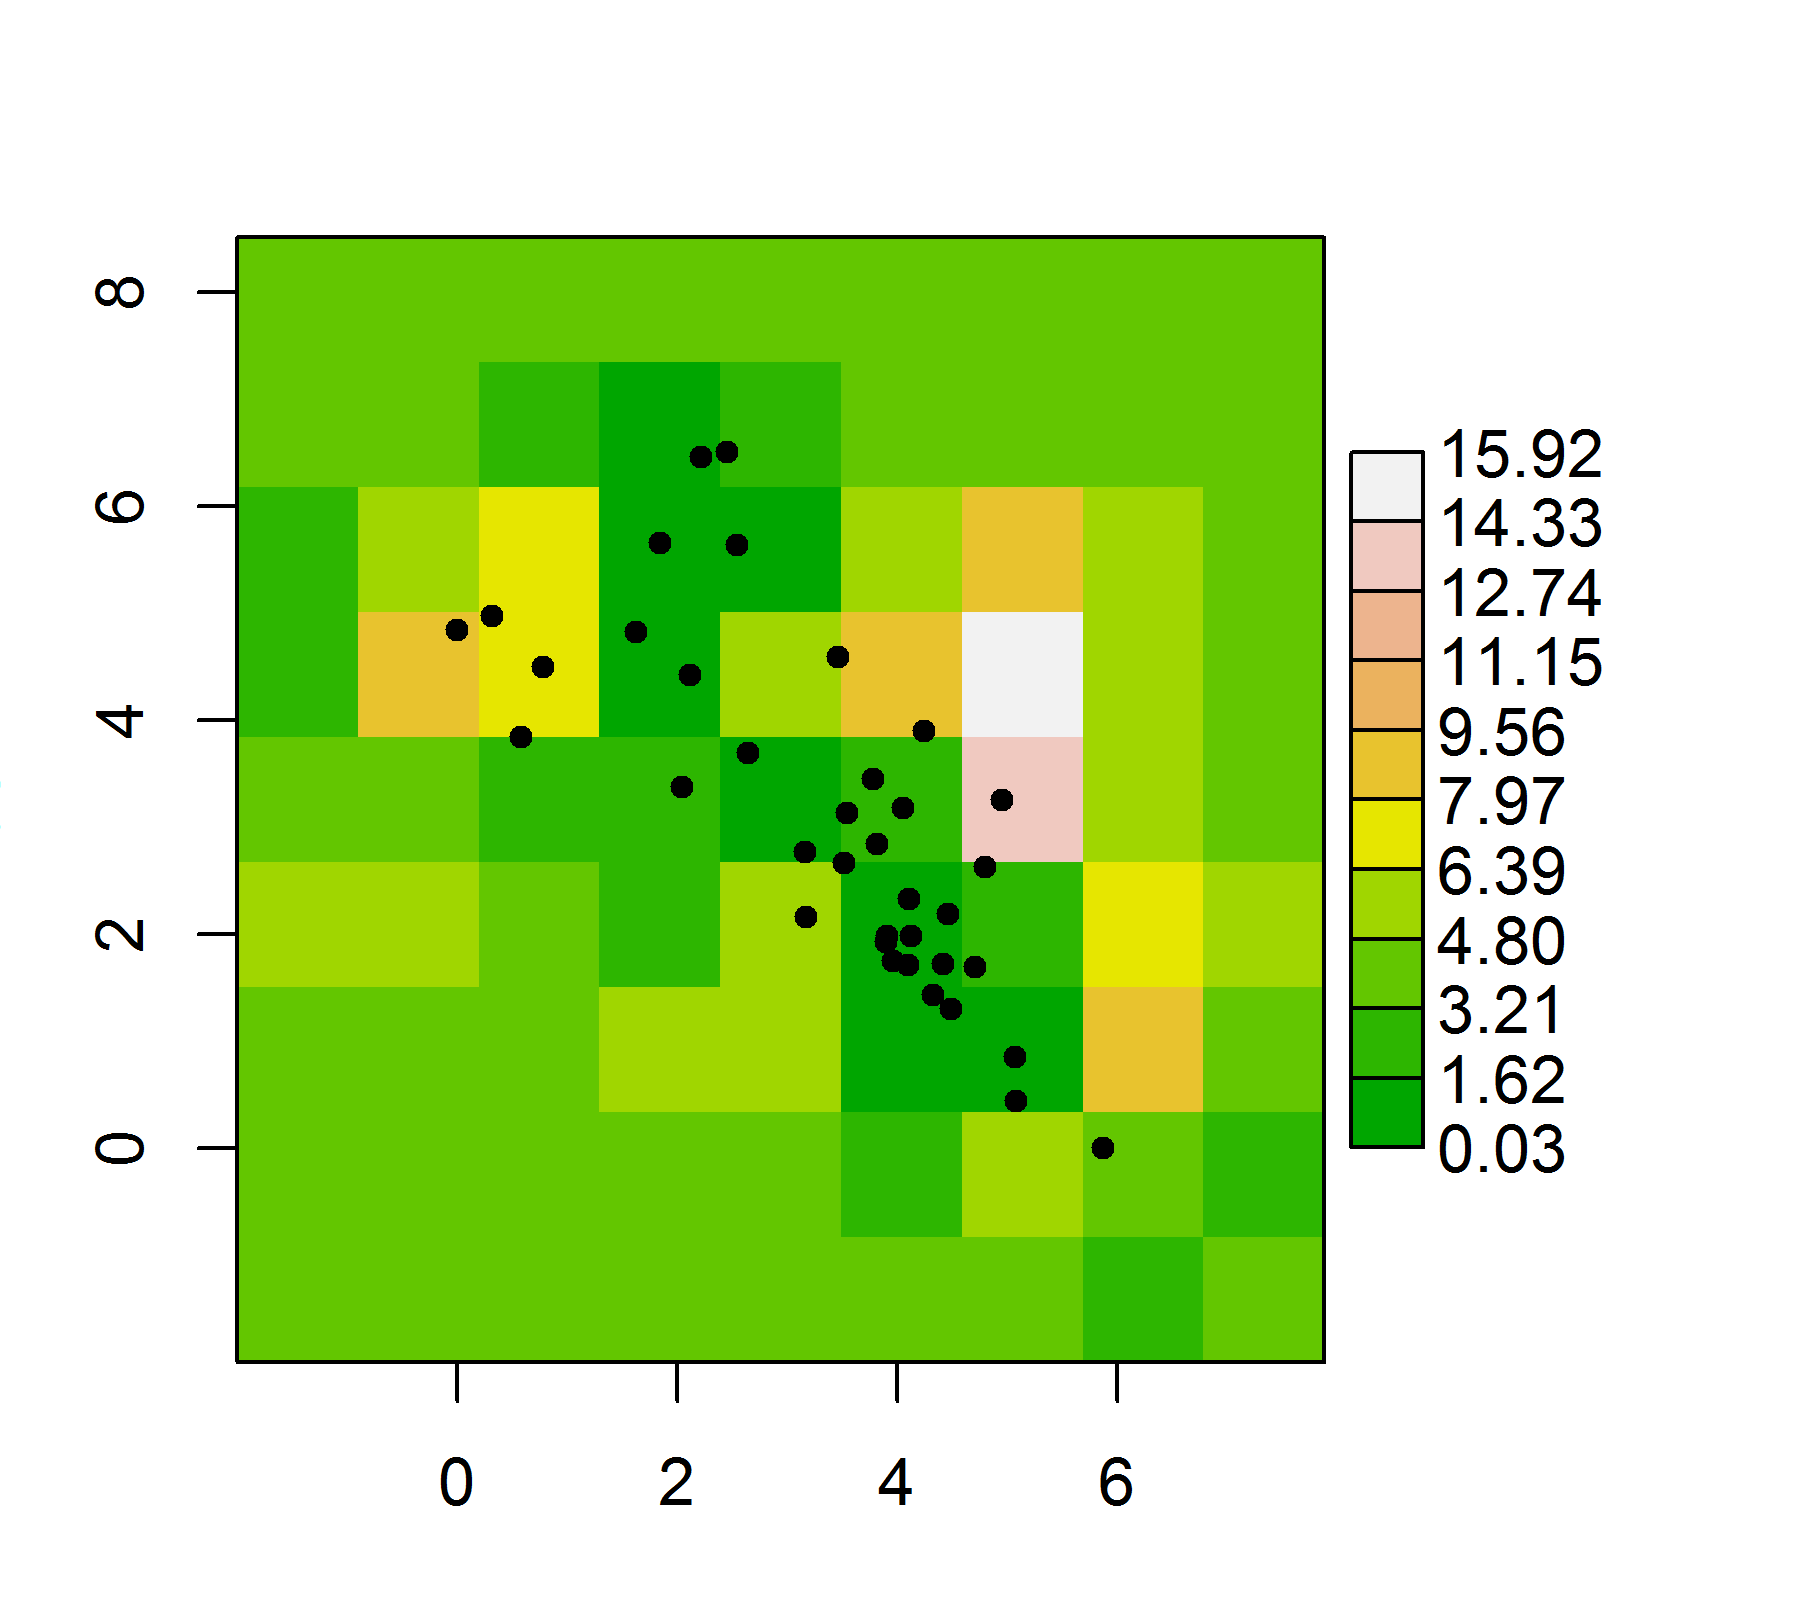
\includegraphics[height=3in,width=3.375in]{Ch4/figs/density10x10}
\end{center}
\caption{Density of wolverines (individuals per 100 $km^2$) in SE Alaska in 2007 based on
  model SCR0. Map grid cells are about 103.7 $km^2$ in area. Dots are the estimated activity centers of the  observed individuals.}
\label{scr0.fig.density10x10}
\end{figure}

\begin{figure}
\begin{center}
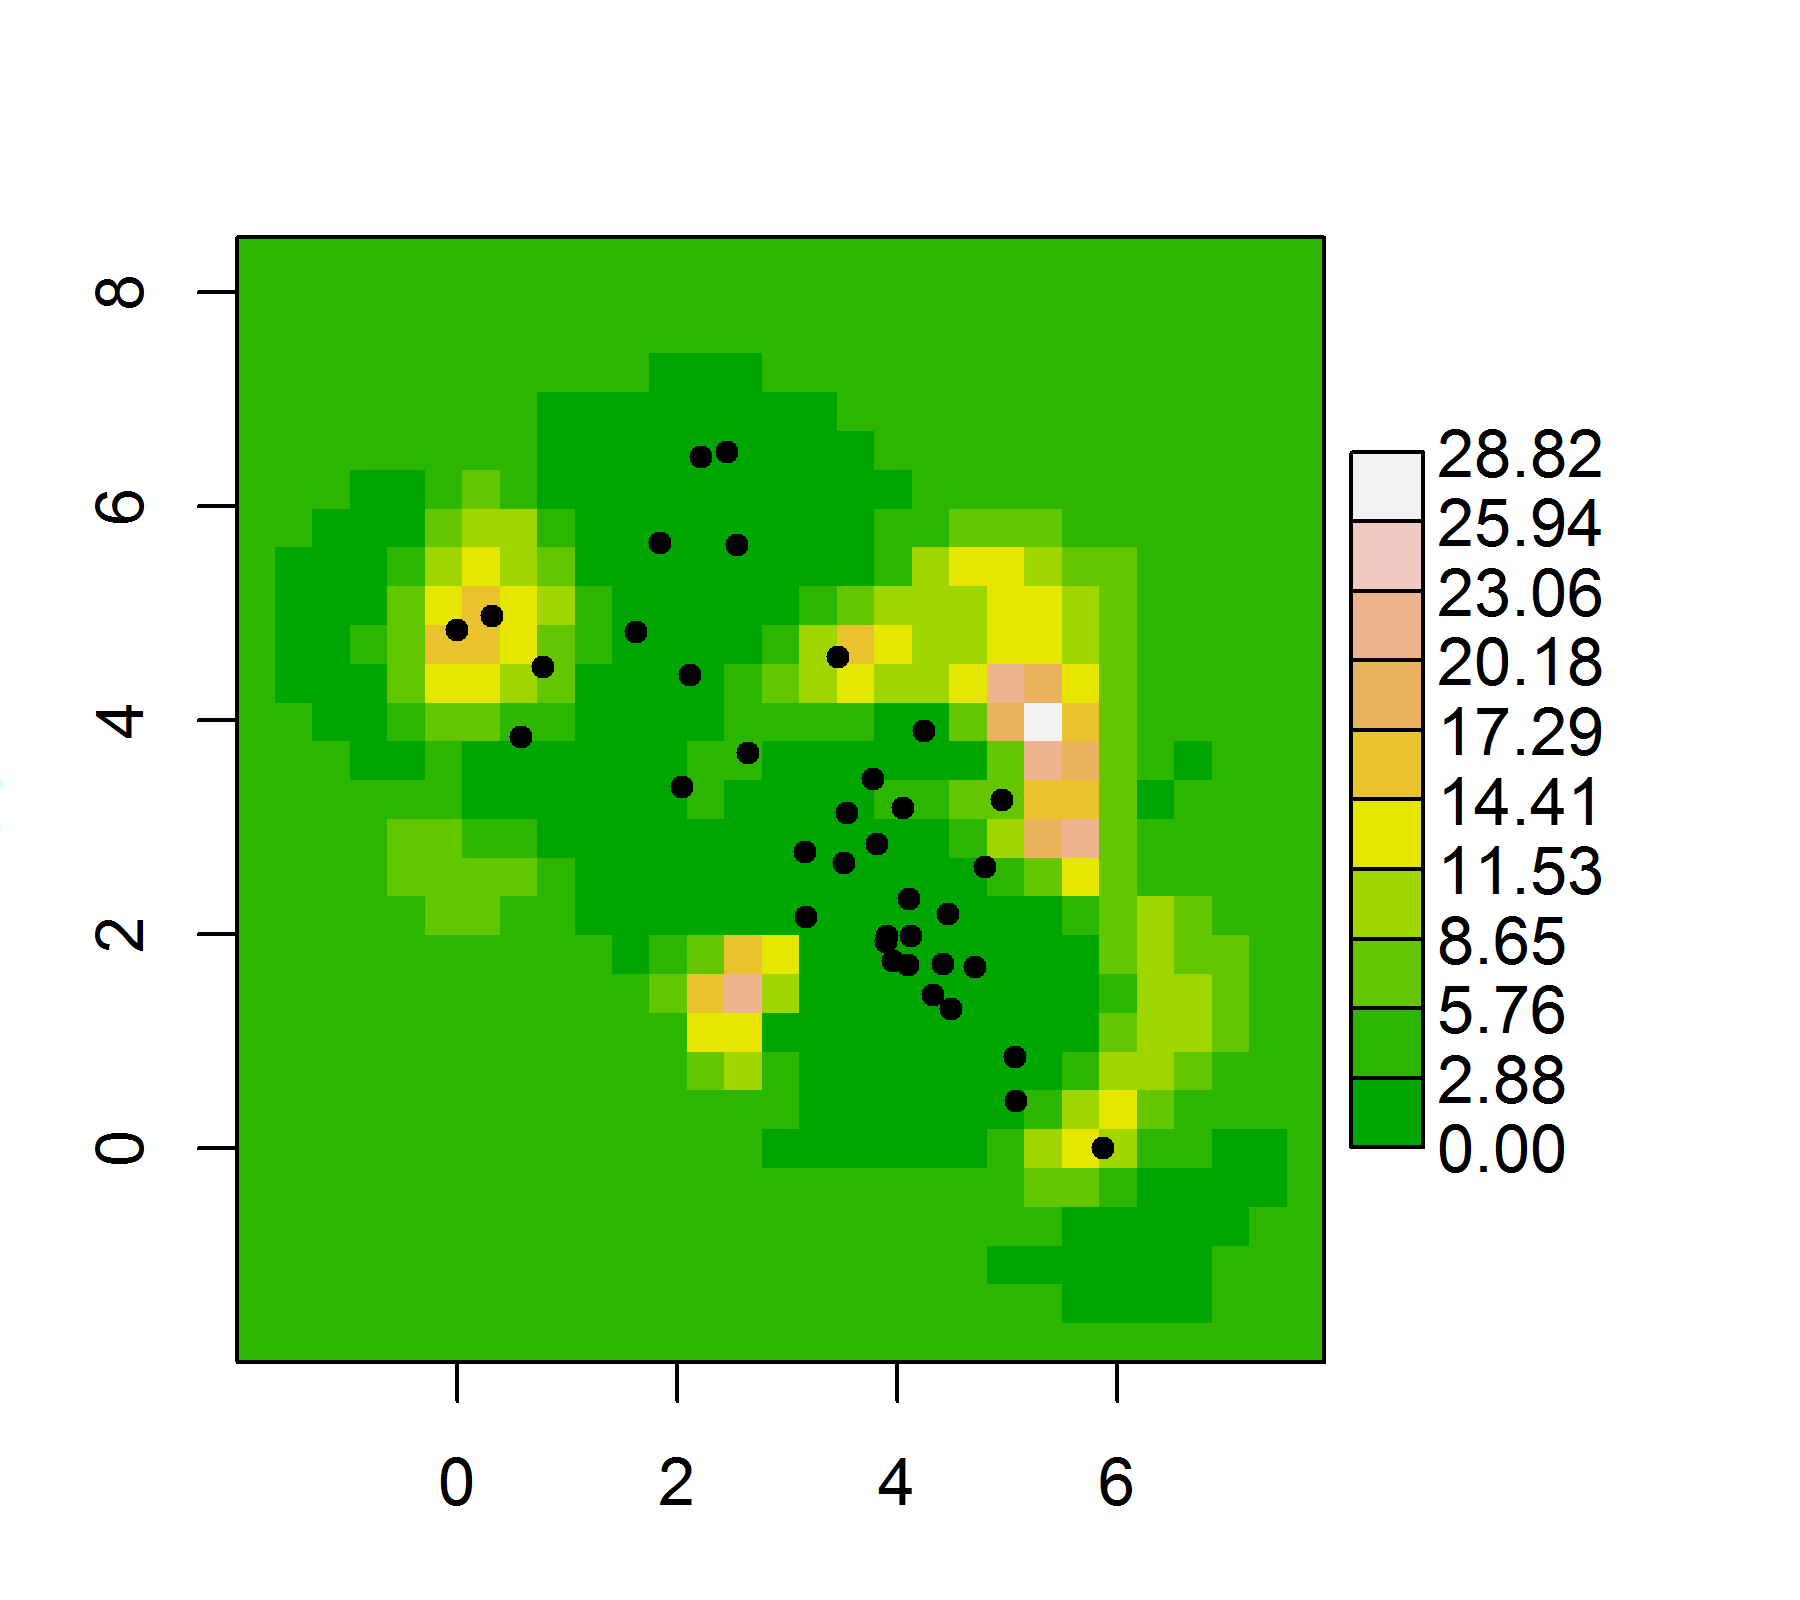
\includegraphics[height=3in,width=3.375in]{Ch4/figs/density30x30}
\end{center}
\caption{Density of wolverines (individuals per 100 $km^2$) based on
  model SCR0. Map grid cells are about 11.5 $km^2$ in area.}
\label{scr0.fig.density20x20}
\end{figure}
XXXXX 
I would combine Fig. 4.4 and 4.5 in a single two-panel plot and call the plot ?Comparison of the effects of pixel size ...?

Then, I would turn color code upside down. I find it more natural to have darker mean a higher value
in the scale , one digit is enough

In Fig. 4.5., I find it funny how the estimated high-density areas are
mostly away from the HR centers of the observed individuals
XXXXXXX

\section{Using a Discrete State-Space to Mask Habitat}
\label{scr0.sec.discrete}

The SCR model developed previously in this chapter assumes that
individual activity centers are distributed uniformly over the
prescribed state-space. Clearly this will not always be a reasonable
assumption. In Chapt. \ref{chapt.state-space} we talk about developing
models that allow explicitly for non-uniformity of the activity
centers by modeling covariate effects on density. A simpler method of
affecting the distribution of activity centers, which we address here,
is to modify the shape and organization of the state-space
explicitly. For example, we might be able to classify the state-space
into distinct blocks of habitat and non-habitat. In that case we can
remove the non-habitat from the state-space and assume uniformity of
the activity centers over the remaining portions judged to be suitable
habitat.  There are several ways to approach this: We can use a
regular grid of points to represent the state-space, i.e., by the set
of coordinates ${\bf s}_1, \ldots, {\bf s}_{G}$, and assign equal
probabilities to each possible value. Alternatively, we can retain the
continuous formulation of the state-space but attempt to describe
constraints analytically, or we can use polygon clipping methods to
enforce constraints on the state-space in the MCMC analysis. We focus
here on the formulation of the basic SCR model in terms of a discrete
state-space but later on (Chapt. \ref{chapt.mcmc} and also Appendix
XYZ) we demonstrate the latter approach based on using polygon
operations to define an irregular state-space.

Use of a discrete state-space can be computationally expensive in {\bf
  WinBUGS}. That said, it isn't too difficult to do the MCMC
calculations in {\bf R} which we discuss briefly in Chapt.
\ref{chapt.mcmc}. The {\bf R} package {\tt SPACECAP}
\citep{gopalaswamy_etal:2011} arose from the {\bf R} implementation of
the SCR model in \citet{royle_etal:2009}.  As we will see in
Chapt. \ref{chapt.mle}, we must prescribe the state-space by a
discrete mesh of points in order to do integrated likelihood and so if
we are using a discrete state-space this can be accommodated directly
in our code for obtaining MLEs.

While clipping out non-habitat seems like a good idea, we think
investigators should go about this very cautiously.  We might prefer
to do it when non-habitat represents a clear-cut restriction on the
state-space such as a reserve boundary or a lake, ocean or river. But,
having the capability to do this also causes people to start defining
``habitat'' vs. ``non-habitat'' based on their understanding of the
system whereas it can't be known whether the animal being studied has
the same understanding.  Moreover, differentiating the landscape by
habitat or habitat quality must affect the geometry and morphology of
home ranges (see Chapt. \ref{chapt.rsf}) much more so than the
plausible locations of activity centers. That is, a home range
centroid could, in actual fact, occur in a Walmart parking lot if
there is pretty good habitat around walmart, so there is probably no
sense to cut out the Walmart lot and preclude it as the location for
an activity center.  It would generally be better to include some
definition of habitat quality in the model for the detection
probability \citep{royle_etal:2012ecol} which we address in
Chapts. \ref{chapt.rsf} and \ref{chapt.ecoldist}.

XXXXXX Andy stopped here XXXXXXXXXXXXXX

\subsection{Evaluation of Coarseness of Discrete Approximation}

The coarseness of the state-space should not really have much of an
effect on estimates if the grain is sufficiently fine relative to
typical animal home range sizes.  Why is this?  We have two analogies
that can help us understand this. First is the relationship to model
$M_{h}$.  As noted in sec. \ref{scr0.sec.scrmh} above, we can think
about SCR models as a type of finite mixture
\citep{norris_pollock:1996, pledger:2000} where we are fortunate to be
able to obtain direct information about which group individuals
belong to (group being location of activity center).  In the standard
finite mixture models we typically find that only 1 or a very small
number of groups (e.g., 2 or 3 at the most) can explain really high
levels of heterogeneity and are adequate for most data sets of small
to moderate sample sizes. We therefore expect a similar effect in SCR
models when we discretize the state-space.
We can also
think about discretizing the state-space as being related
to numerical integration where we find (see
Chapt. \ref{chapt.mle}) that we don't need a very fine
grid of support points to evaluate the integral to a reasonable
level of accuracy. We demonstrate this here by reanalyzing simulated
data using a state-space defined by a different numbers of support points.
We provide an {\bf R} script called \mbox{\tt SCR0bayesDss.fn} in the
{\bf R} package \mbox{\tt scrbook}.  We note that for this comparison
we generated the actual activity centers as a continuous random
variable and thus the discrete state-space is, strictly speaking, an
approximation to truth. That said, we regard all state-space
specifications as approximations to truth in the sense that they
represent a component of the SCR model.
Thus the use of any
specific discrete state-space is not intrinsically more ``wrong'' than
any specific continuous representation.

As with our {\bf R} function \mbox{\tt SCR0bayes}, the modification
\mbox{\tt SCR0bayesDss} will use either {\bf WinBUGS} or {\bf
  JAGS}. In addition, it requires a grid resolution argument
(\mbox{\tt ng}) which is the square-root of the number of points in
the state-space grid.
To execute this function we do, for example:
{\small
\begin{verbatim}
library("scrbook")
data<-simSCR0.fn(discard0=TRUE,sd=2013)   # generate data set
out1<-SCR0bayesDss(data,ng=8,M=200,engine="jags",ni=2000,nb=1000) # JAGS
out2<-SCR0bayesDss(data,ng=8,M=200,engine="winbugs",ni=2000,nb=1000) # WinBUGS
\end{verbatim}
}
We fit this model to the same simulated data set for 
$6 \times 6$, $9 \times 9$, $12 \times 12$, $15\times 15$,
$20\times 20$, $25 \times 25$ and $30 \times 30$ state-space grids.
We used 2000 burn, 12000 total iters with 3 chains, yielding a total
of 30000 posterior samples.
For {\bf WinBUGS}, which takes considerably more time (see below),
 we used 3 chains of 5k total with 1k burnin means 12k
total posterior samples.
Summary results for these analyses are shown in
Table XYZ\footnote{To finish later}.

\begin{verbatim}
Table XYZ.Effect of grid coarseness on estimates of N using JAGS and
WinBUGS.

$I would only show results from one engine. COuld simply say in the text that WB was about 5x slower$
JAGS run from rjags
             Mean       SD    NaiveSE  Time-seriesSE  runtime
6    N     109.7717 15.98959 0.0923160    0.377737    1239
9    N     114.4621 16.72025 0.0965344    0.468659    1267
12   N     115.4309 17.12403 0.098866     0.464830    1576
15   N     114.7699 17.0242  0.0982894    0.425238    1638
20   N     116.0370 17.10686 0.0987665    0.486867    1647
25   N     116.3228 16.98323 0.0980527    0.465527    1661
30   N     116.4252 17.4078  0.100504     0.533735    1806
WinBUGS run from R2WinBUGS
             Mean       SD    NaiveSE  Time-seriesSE  runtime
6    N     111.6699 16.61414 0.1516657   0.682008     2274
9    N     114.2294 17.99109 0.1642355   0.833291     4300
12   N     115.9806 17.3843  0.1586964   0.762756     7100
15   N     115.379  17.93721 0.1637436   0.832483    13010

Note: WinBUGS based on fewer samples too!
\end{verbatim}

The results in terms of the posterior summaries are, as we
expect, very similar using {\bf WinBUGS}. However, it was interesting
to note that {\bf WinBUGS} runtime is much worse (note the number of
iterations is lower for {\bf WinBUGS} yet the runtime is much longer)
and, furthermore, it seems to scale with the size of the
discrete state-space grid. While that was expected, it was unexpected
that the runtime of {\bf JAGS} would seem relatively consistent
as we increase the grid size.
We suspect that {\bf WinBUGS} is evaluating the full-conditional for
each activity center at all $G$ possible values whereas it may be that
{\bf JAGS} is evaluating the full-conditional only at a subset of
values or perhaps using previous calculations more effectively.

While this might suggest that one should always use {\bf JAGS} for
this analysis, we found in our analysis of the wolverine (next
section) that {\bf JAGS} could be extremely sensitive to starting
values, producing MCMC algorithms that sometimes simply did not work.

\subsection{Analysis of the wolverine camera trapping data}


We reanalyzed the wolverine data using discrete state-space grids with
points spaced by 2, 4 and 8 km (see in
Fig. \ref{scr0.fig.wolvgrids}). These were constructed from a 40 km
buffered state-space, and deleting the points over water
\citep[see][]{royle_etal:2011jwm}.  Our interest in doing this was to
evaluate the relative influence of grid resolution on estimated
density because the coarser grids will be more efficient from a
computational stand-point and so we would prefer to use them, but
only if there is no strong influence on estimated density.
The density estimates are only slightly different (xxxxsay in which wayxxxxx)is a bit different depending on the grid size. Also the
effectiveness of the MCMC algorithms is pretty remarkably
different. The 2km grid took 6 days to run!

\begin{figure}
\begin{center}
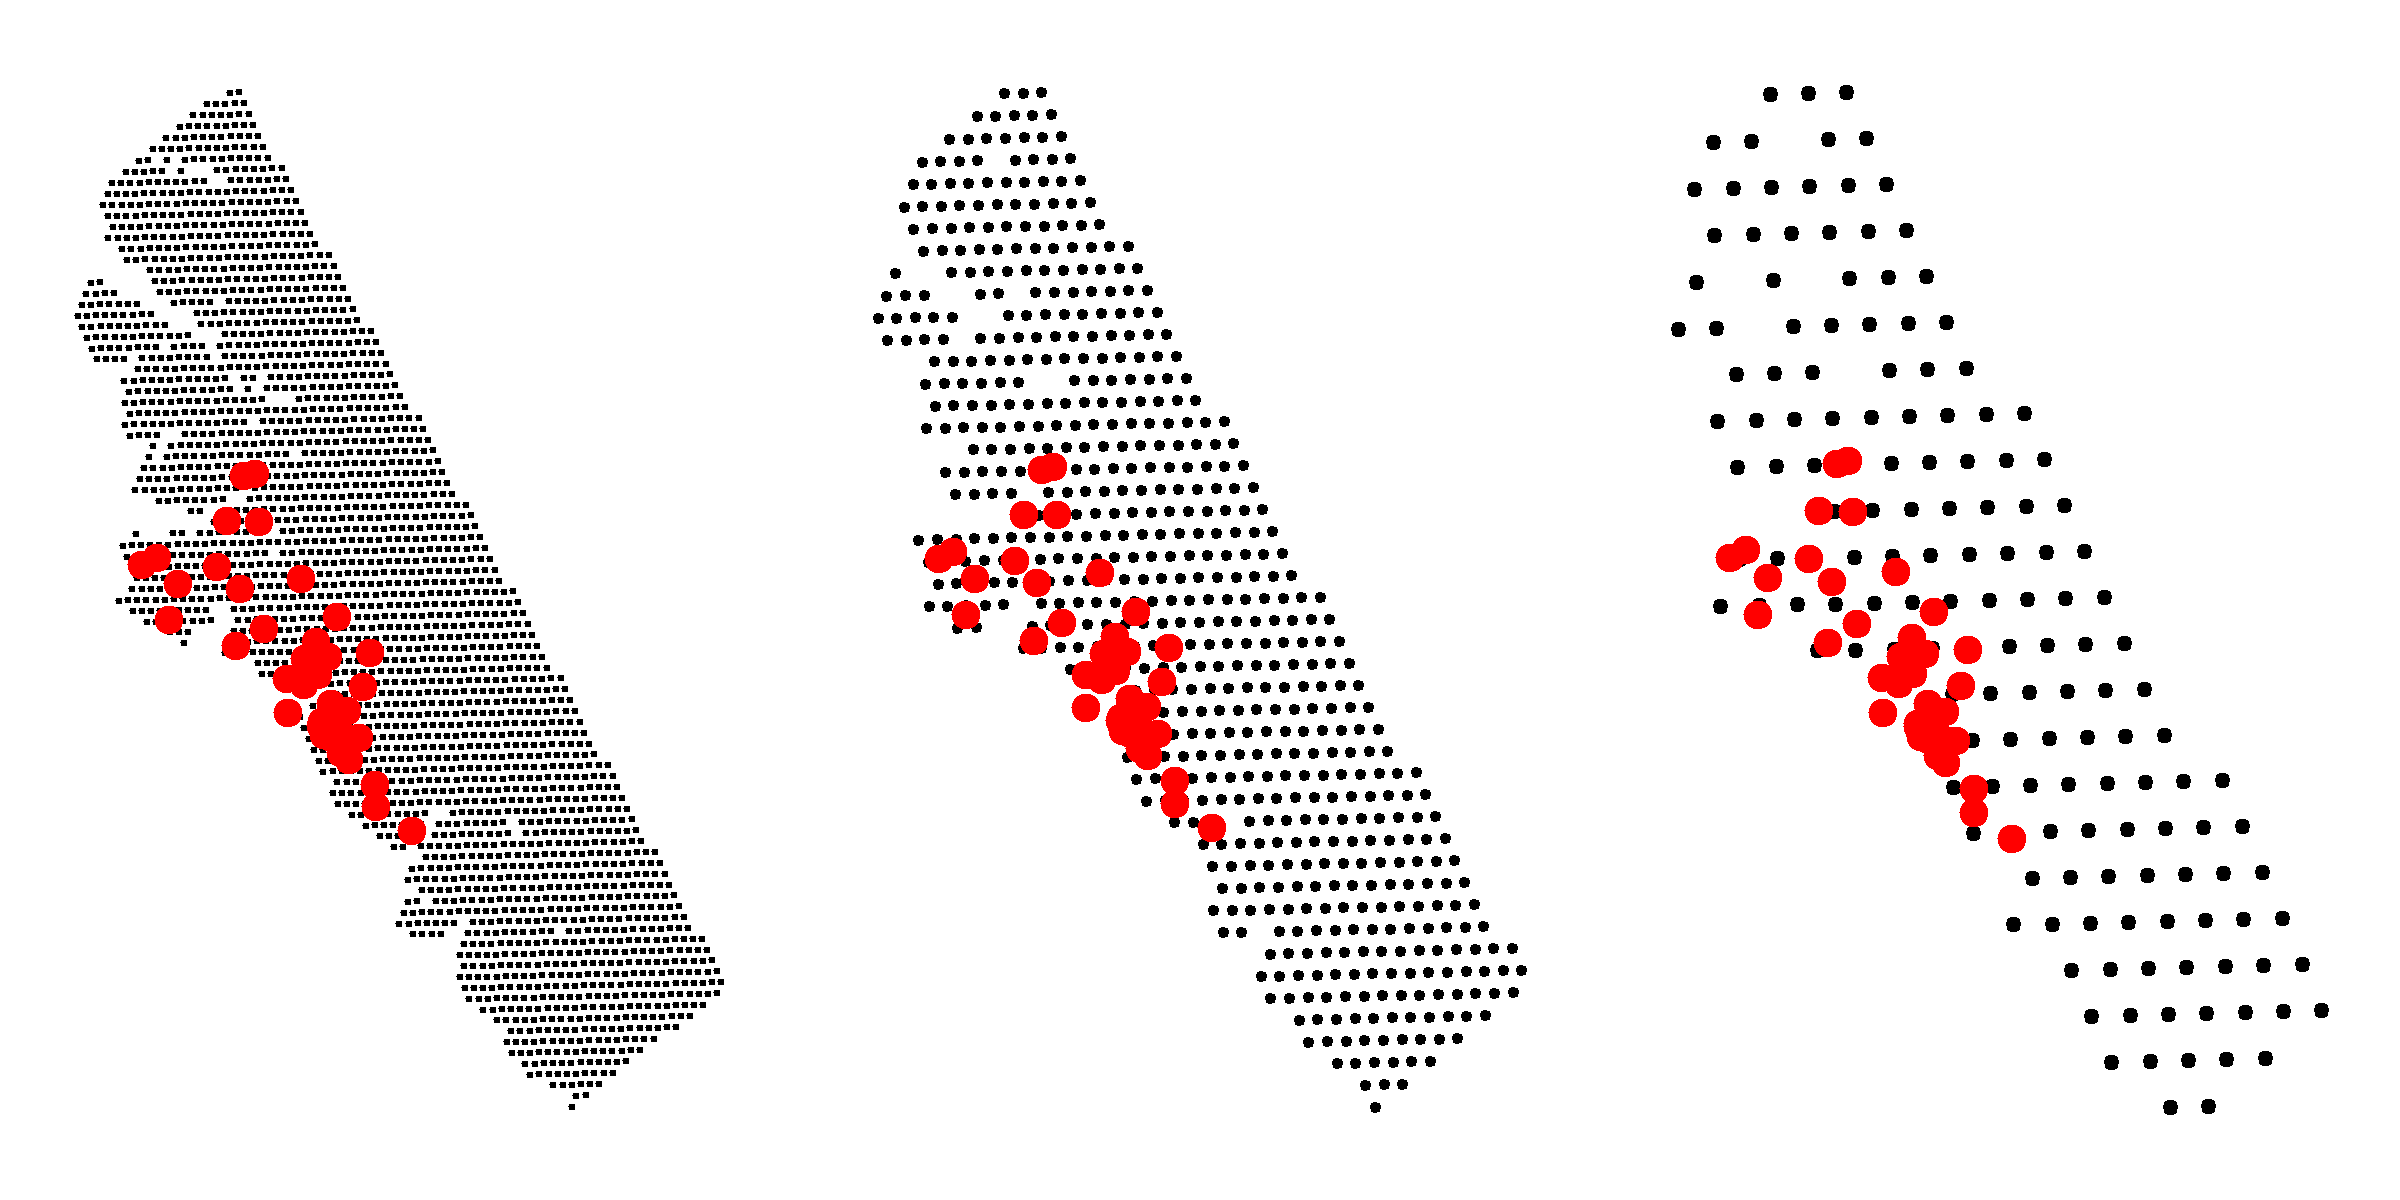
\includegraphics[height=2.5in,width=5in]{Ch4/figs/wolvgrids}
\end{center}
\caption{Comparison of the effect of pixel size on the estimated density surface of wolverine sin SE Alaska 2007. Xxxxxx 2 km 4 km and 8km wolverine state-space grids extending about
40 km from the vicinity of the trap array. }
\label{scr0.fig.wolvgrids}
\end{figure}

{\small
\begin{verbatim}
This will be summarized in a table

> print(out.2km,digits=2)
Inference for Bugs model at "modelfile.txt", fit using WinBUGS,
 3 chains, each with 11000 iterations (first 1000 discarded)
 n.sims = 30000 iterations saved
       mean    sd  2.5%   25%   50%   75%  97.5% Rhat n.eff
psi    0.43  0.09  0.27  0.37  0.43  0.49   0.63 1.00   560
sigma  0.62  0.05  0.54  0.59  0.62  0.65   0.73 1.01   160
lam0   0.05  0.01  0.04  0.04  0.05  0.06   0.07 1.01   320
p0     0.05  0.01  0.03  0.04  0.05  0.05   0.06 1.01   320
N     86.56 16.94 57.00 75.00 85.00 97.00 124.00 1.00   510
D      8.78  1.72  5.78  7.60  8.62  9.83  12.57 1.00   510

For each parameter, n.eff is a crude measure of effective sample size,
and Rhat is the potential scale reduction factor (at convergence, Rhat=1).
> print(out.4km,digits=2)
Inference for Bugs model at "modelfile.txt", fit using WinBUGS,
 3 chains, each with 11000 iterations (first 1000 discarded)
 n.sims = 30000 iterations saved
       mean    sd  2.5%   25%   50%    75%  97.5% Rhat n.eff
psi    0.45  0.09  0.28  0.38  0.44   0.50   0.64    1  1300
sigma  0.61  0.04  0.53  0.58  0.61   0.64   0.71    1  1600
lam0   0.05  0.01  0.04  0.05  0.05   0.06   0.07    1  2500
p0     0.05  0.01  0.03  0.04  0.05   0.05   0.07    1  2500
N     89.25 17.44 59.00 77.00 88.00 100.00 127.00    1  1100
D      9.01  1.76  5.96  7.77  8.88  10.10  12.82    1  1100

For each parameter, n.eff is a crude measure of effective sample size,
and Rhat is the potential scale reduction factor (at convergence, Rhat=1).
> print(out.8km,digits=2)
Inference for Bugs model at "modelfile.txt", fit using WinBUGS,
 3 chains, each with 11000 iterations (first 1000 discarded)
 n.sims = 30000 iterations saved
       mean    sd  2.5%   25%   50%   75%  97.5% Rhat n.eff
psi    0.42  0.09  0.26  0.36  0.41  0.47   0.61 1.00   940
sigma  0.68  0.05  0.59  0.64  0.67  0.71   0.77 1.01   220
lam0   0.05  0.01  0.03  0.04  0.05  0.05   0.06 1.00   560
p0     0.05  0.01  0.03  0.04  0.04  0.05   0.06 1.00   560
N     83.18 16.14 56.00 72.00 82.00 93.00 119.00 1.00   700
D      8.28  1.61  5.57  7.17  8.16  9.26  11.84 1.00   700

For each parameter, n.eff is a crude measure of effective sample size,
and Rhat is the potential scale reduction factor (at convergence, Rhat=1).
\end{verbatim}
}


\begin{comment}
We did the analysis in JAGS also. The results are shown below. {\bf Note}: I
am going to run these again but for longer to finalize the results.

{\small
\begin{verbatim}
 ### 01/10/2012 -- need to rerun these JAGS runs but use more
iterations and check results.


2km
Iterations = 7001:13000
Thinning interval = 1
Number of chains = 3
Sample size per chain = 6000

          Mean        SD  Naive SE Time-series SE
N     86.28522 16.950626 1.263e-01      0.4878973
lam0   0.04807  0.007512 5.599e-05      0.0002199
p0     0.04581  0.006820 5.083e-05      0.0001996
psi    0.28904  0.062117 4.630e-04      0.0017481
sigma  0.62769  0.043596 3.249e-04      0.0018724

4km
          Mean        SD  Naive SE Time-series SE
N     85.53139 16.998966 1.267e-01      0.5181297
lam0   0.04636  0.007542 5.621e-05      0.0002382
p0     0.04425  0.006867 5.118e-05      0.0002172
psi    0.28650  0.061922 4.615e-04      0.0018276
sigma  0.64281  0.048321 3.602e-04      0.0022911

8km
          Mean        SD  Naive SE Time-series SE
N     83.97039 16.508146 1.230e-01      0.4548782
lam0   0.04519  0.006919 5.157e-05      0.0001738
p0     0.04319  0.006319 4.710e-05      0.0001589
psi    0.28146  0.060653 4.521e-04      0.0016555
sigma  0.66956  0.040989 3.055e-04      0.0015070
\end{verbatim}
}
\end{comment}




\begin{comment}


\subsection{SCR models as multi-state models}

While we invoke a discrete state-space artificially, by gridding the
underlying continuous state-space, sometimes the state-space is more
naturally discrete. Consider a situation in which discrete patches of
habitat are searched using some method and it might be convenient (or
occur inadvertently) to associate samples to the patch level instead
of recording observation locations. In this case we might use a model
${\bf s}_{i} \sim dcat(probs[])$  where $probs[]$ are the probabilities that
an individual inhabits a particular patch. We consider such a case
study in Chapt. XX Poisson XXX from \citet{mollet_etal:2012} who
obtained a population size estimate of a large grouse species known as
the capracaillie. Forest patches were searched for scat which was
identified to individual by DNA analysis.
Even when space is {\it not}
naturally discrete, measurements are often made at a fairly coarse
grain (e.g., meters or tens of meters along a stream), or associated
with spatial quadrats for scat searches and therefore the state-space
may be effectively discrete in many situations.

This discrete formulation of SCR models suggests that SCR models are
related to ordinary multi-state models \citep[][ch. 9]{kery_schaub:2011}
which are also parameterized in terms of a discrete state
variable which is often defined as a spatially-indexed state related
either to location of capture or breeding location. While many
multi-state models exist in which the state variable is not related to
space, multi-state models have been extremely useful in development
models of movements among geographic states and indeed this type of
problem motivated their early developments by \citet{arnason:1972,
  arnason:1973} and \citet{hestbeck_etal:1991}.  We pursue this
connection a little bit more in chapter XXX XYZ.

\end{comment}



\section{ Summary and Outlook }

We have emphasized throughout this chapter that the basic SCR
model is an ordinary capture-recapture model for
closed populations, but augmented with a set
of latent individual effects , ${\bf s}_{i}$, which relate encounter
probability to some sense of individual location. SCR models are
therefore a type of individual covariate model (as introduced in
chapter \ref{chapt.closed}) -- but with imperfect information about the
individual covariate. In other words, they are GLMM-type of models.
 Another class of capture-recapture models
that SCR models are closely related to is the so-called ``model
$M_{h}$'' \citep{otis_etal:1878, dorazio_royle:2002}.
The effect of introducing a spatial location for individuals is that
it induces heterogeneity in detection probability, as in model
$M_{h}$. However, unlike model $M_{h}$, we obtain some information
about the individual effect which is completely latent in model
$M_{h}$. If the state-space of the random effect ${\bf s}$ is discrete,
the SCR model resembles more closely the finite-mixture 
heterogeneity models \citep{norris_pollock:1996} which parameterizes
heterogeneity by assuming that individuals belong to discrete classes
or groups (e.g., having high, medium, low values of encounter probability). In the context of SCR models we
obtain some information about the group membership  in the
locations where individuals are captured.  Given the direct
relationship of SCR models with so many standard classes of models, we
find that they are really quite easy to analyze using standard MCMC
methods encased in black boxes such as {\bf WinBUGS} or {\bf JAGS} and
no doubt other packages. They are also easy to analyze using classical
likelihood methods, which we address in Chapt. \ref{chapt.mle}.

One of the things we've introduced in this chapter which has not
previously been discussed explicitly in the literatre on SCR models,
is the manner in which the encounter probability model relates to
space usage of individuals. Thats kind of a BFD. XXX SPACE USAGE XXXX

xxxxxx$In the next I find hard to understand the difference between the uniformity of the prior for the activity center locations and the non-uniformity of their posterior. What excatly is the relevance of that ? What is the difference between this and any other Bayesian analysis, where we have also usually an assumption like ?uniformity? about where something (typically a parameter value) sits and then after incorporating the information in the data, this ?space? (the posterior) is no longer uniform. Not sure whether this makes sense ... ?$ xxxxxxFormal consideration of the collection of individual locations $({\bf
  s}_{1}, \ldots, {\bf s}_{N})$ in the model is fundamental to all of
the models considered in this book. In statistical terminology, we
think of the collection of points $\{ {\bf s}_{i} \}$ as a realization of a
point process and part of the promise, and ongoing challenge, of SCR
models is to develop models that reflect interesting biological
processes, for example interactions among points or temporal dynamics
in point locations.  Here we considered the simplest possible point
process model - the points are independent and uniformly
(``randomly'') distributed over space. Despite the simplicity of this
assumption, it should suffice in many applications of SCR models
although we do address generalizations of this model in later
chapters. Moreover, even though the {\it prior} distribution on the
point locations is uniform, the realized pattern may deviate markedly
from uniformity as the observed encounter data provide information to
impart deviations from uniformity. Thus, the estimated density map
will typically appear distinctly non-uniform.  As a general rule,
information in the data will govern estimates of individual point
locations so even fairly complex patterns of non-independence or
non-uniformity will appear in the data. That is, we find in
applications of the basic SCR model that this simple {\it a priori}
model can effectively reflect or adapt to complex realizations of the
underlying point process.  For example, if individuals are highly
territorial then the data should indicate this in the form of
individuals not being encountered in the same trap - the resulting
posterior distribution of point locations should therefore reflect
non-independence.  Obviously the complexity of posterior estimates of
the point pattern will depend on the quantity of data, both number of
individuals and captures per individual.  Because the point process is
such an integral component of SCR models, the state-space of the point
process plays an important role in developing SCR models. As we tried
to emphasize in this chapter, the choice of the state-espace is part of
the model. It can have an influence on parameter estimates and other
inferences such as model selection (see chapter \ref{chapt.gof}). We
emphasize however that this is not an arbitrary decision like
``buffering'' because the model induces an explicit interpretation of
parameters and statistical effect on estimators xxxxx$what does this mean ?$xxxxxx.

We showed how to conduct Bayesian inference about the underlying point process
including calculation of density maps from posterior output. We can do
other things we normally do with spatial point processes such as
compute K-functions xxxx$need references for such things$ xxxxxxand test for ``complete spatial randomness''
(CSR) which we develop in Chapt.  \ref{chapt.gof}. 


\begin{comment}
xxxxx$I would tone down the next paragraph. Also, after having read this chapter (and understood at least the main things in it), this question does not strike me as very obvious anymore$ xxxxxAn obvious question that might be floating around in your mind is why
should we ever go through all of this trouble when we could just use
{\bf MARK} or {\bf CAPTURE} xxx$this bold face is intrusive on the eye$ xxxxxto get an estimate of $N$ and apply $1/2$
MMDM methods?  The main reason is that these conventional methods are
predicated on models that represent explicit misspecifications of both
the observation and ecological process - they are wrong!  Not just
wrong, because of course all models are wrong, but they're not even
{\it plausible} models! Thus while we might be able to show adequate
fit or whatever, we think as a conceptual and philosophical model one
should not be using models that are not even plausible data-generating
models -- even if the plausible ones don't fit!  Perhaps more
charitably, these ordinary non-spatial models are models of the wrong
system. They do not account for trap identity. They don't account for
spatial organization or clustering of individual encounters in
space. And, density is not estimable from such models because 
it has no meaning absent an explicit representation of space. If
we do define space explicitly, e.g., as a buffered minimum convex
hull, then the normal models ($M_{0}$, $M_{h}$, etc..) assume that
individual capture-probability is not related to space, no matter how
we define the buffer.  Conversely, the SCR model is a model for
trap-specific encounter data - how individuals are organized in space
and interact with traps. SCR models provide a coherent framework for
inference about density or population size and also, because of the
formality of their derivation, can be extended and generalized to a
large variety of different situations, as we demonstrate in subsequent
chapters.
\end{comment}

In the next few chapters we continue to work with this basic SCR
design and model but consider some important extensions of the basic
model.  For example, we consider
extensions
to  include covariates that vary by individual, trap, or over time
(Chapt.  \ref{chapt.covariates}), spatial covariates on density
(Chapt.  \ref{chapt.state-space}),
 open populations (Chapt. \ref{chapt.open}), model assessment and
 selection (Chapt. \ref{chapt.gof}) and other topics.
We also consider technical details of Bayesian (Chapt. 
\ref{chapt.mcmc}) and  maximum
likelihood (Chapt.  \ref{chapt.mle}) estimation so that the interested
reader can develop or extend their own methods to suit their needs.
